\documentclass[preprint,12pt,authoryear]{elsarticle}

% Math
\usepackage{amsmath,amssymb,amsfonts,mathtools}

% Typography and figures
\usepackage[utf8]{inputenc}
\usepackage[T1]{fontenc}
\usepackage{booktabs}
\usepackage{multirow}
\usepackage{graphicx}
\graphicspath{{figures/}}
\usepackage{subcaption}
\usepackage{placeins}
\usepackage{xcolor}
\usepackage{url}
\usepackage{microtype}
\usepackage{hyperref}
\usepackage[capitalize,noabbrev]{cleveref}

\journal{Computers and Electronics in Agriculture}

% Commands
\newcommand{\R}{\mathbb{R}}
\DeclareMathOperator*{\argmax}{arg\,max}
\DeclareMathOperator{\softmax}{softmax}
\newcommand{\vx}{\mathbf{x}}
\newcommand{\vr}{\mathbf{r}}
\newcommand{\vp}{\mathbf{p}}
\newcommand{\vh}{\mathbf{h}}
\newcommand{\vz}{\mathbf{z}}
\newcommand{\vl}{\mathbf{l}}
\newcommand{\cL}{\mathcal{L}}
\newcommand{\ours}{TIM}
\newcommand{\task}{Agricultural Machinery Trajectory Time-Series Classification}

\begin{document}

\begin{frontmatter}

\title{\ours{}: Trajectory-ViT-Audio Multimodal Learning for Eleven-Class \task{}}

\author[caus]{Zhou Guo}
\address[caus]{College of Information and Electrical Engineering, China Agricultural University, Beijing 100083, China}

\begin{abstract}
\task{} aims to infer machinery operation states from time-indexed sensor records, supporting operation monitoring, efficiency evaluation, and data-driven farm management.
GNSS trajectory methods are effective for field-road discrimination and coarse operational recognition, but they remain limited for fine-grained combine-harvester operations that share overlapping motion patterns in position, speed, heading, curvature, and dwell time.
For these ambiguous states, discriminative evidence often lies in complementary sensor streams: audio captures engine load, idling, unloading, and working-component engagement, whereas images capture crop contact, material flow, harvesting scenes, and field-road context.
However, multimodal use is nontrivial because audio lacks path geometry, images are sensitive to illumination, viewpoint, and occlusion, and the three streams differ in sampling rate, noise characteristics, temporal alignment, and feature space.
This paper studies an eleven-class combine-harvester setting and proposes \ours{}, a multimodal model that integrates trajectory, ViT visual, and audio streams for \task{}.
\ours{} encodes causal GNSS trajectories, synchronized ViT visual frames, and acoustic spectrograms with modality-specific branches, then applies class-adaptive logit-level fusion to combine motion, scene, and process cues under a unified classification objective.
Experiments are conducted on a real-world dataset collected over three months of maize harvest operations in Ningxia, Shaanxi, and Inner Mongolia.
On the held-out test set, \ours{} achieves 81.36\% accuracy, 63.64\% macro-F1, and 81.01\% weighted-F1, exceeding the strongest unimodal baseline by 9.00 macro-F1 points.
Compared with direct trimodal concatenation, the class-adaptive gate improves accuracy, macro-F1, and weighted-F1 by 2.21, 2.44, and 2.56 percentage points, respectively.
Per-class analysis shows that \ours{} improves 8 of 11 operation classes over the best single modality, with large gains for reverse transfer, turning transfer, and idling waiting, while unloading and road driving remain challenging.
To the best of our knowledge, this is the first synchronized trajectory, ViT visual, and audio study of eleven-class \task{}.

\end{abstract}

\begin{keyword}
Agricultural machinery trajectory time-series classification, multimodal learning, GNSS trajectory, visual classification, audio classification, combine harvester.
\end{keyword}

\end{frontmatter}

\section{Introduction}
\label{sec:intro}

Agricultural machinery has become a central carrier of field-scale production data. Modern combine harvesters continuously record GNSS trajectories, visual observations, and machine sounds while executing harvesting, transfer, waiting, unloading, and road-driving operations. Turning these raw sensor streams into reliable operational labels is the core goal of \task{}. Accurate labels support operation-efficiency evaluation, harvest-loss analysis, machine scheduling, and downstream digital-farm management.

Most prior work treats agricultural machinery trajectory analysis as field-road classification or coarse-grained operational state classification~\cite{pan2024chaos,zhai2024atrnet,zhai2024bilstm}. These settings are important, but they do not capture the operational detail required by real combine-harvester workflows. In this work, we study an eleven-class problem that distinguishes reverse empty harvesting, straight empty harvesting, turning empty harvesting, full-load harvesting, reverse transfer, straight transfer, turning transfer, engine-off waiting, idling waiting, unloading, and road driving.

The main challenge is that several classes are not separable from trajectory geometry alone. Engine-off waiting, idling waiting, and unloading are all nearly stationary in GNSS coordinates. Straight empty harvesting and straight transfer can both appear as smooth linear motion. Turning empty harvesting and turning transfer can have similar curvature. In these cases, the decisive evidence lies outside the trajectory stream: video reveals crop rows, header state, and scene context, while audio reflects engine load, idling, unloading mechanisms, and other process-level cues. This motivates a multimodal formulation of \task{}.

This paper is written around the current controlled multimodal eleven-class classification suite with matched temporal context. The trajectory modality uses a 128-second causal sequence, selected because a completed seq\_len ablation found it to provide the best mean macro-F1 among 64, 128, 256, and 512 seconds. The ViT visual modality follows the same 128-second causal window and selects the nine frames closest to the label time. The audio modality uses AST-based spectrogram encoding. The current \ours{} model replaces direct feature concatenation with class-adaptive logit-level fusion, so that different operation classes can assign different weights to BiLSTM, ViT, and AST evidence.

The contributions of this paper are:
\begin{enumerate}
    \item We formulate an eleven-class \task{} benchmark for combine-harvester operations and define a unified BiLSTM--ViT--AST experimental protocol with matched causal temporal context.
    \item We evaluate modality-specific baselines, including BiLSTM trajectory encoding, pretrained ViT visual encoding with temporal pooling, and AST audio encoding, under a shared split and fixed seed.
    \item We propose a class-adaptive trimodal fusion model that initializes from unimodal checkpoints and combines modality-specific logits with class-wise BiLSTM, ViT, and AST gates, improving fixed-seed macro-F1 by 2.44 percentage points over direct trimodal concatenation.
    \item We provide trajectory-level diagnostic visualizations, per-class confusion analysis, fusion ablations, and sequence-length ablations showing that multimodal fusion improves most harvesting, transfer, and waiting/transfer classes while revealing unloading and road-driving states that remain challenging.
\end{enumerate}

The remainder of this paper is organized as follows. \Cref{sec:related} reviews agricultural machinery trajectory analysis and multimodal learning. \Cref{sec:method} describes the proposed multimodal model. \Cref{sec:exp} presents the dataset, implementation details, and experiments. \Cref{sec:discussion} discusses modality-specific findings and limitations. \Cref{sec:conclusion} concludes the paper.

\section{Related Work}
\label{sec:related}

\subsection{Agricultural Machinery Trajectory Analysis}

GNSS-based trajectory analysis is the dominant foundation for agricultural machinery monitoring. Early and rule-based methods commonly used speed, heading, and field-boundary constraints to distinguish field and road segments. More recent learning-based work improves robustness by modeling temporal structure and trajectory-derived features. Zhai et al.~\cite{zhai2024bilstm} studied sparse agricultural machinery trajectories and used recurrent models to improve trajectory reconstruction and downstream classification. Zhai et al.~\cite{zhai2024atrnet} transformed trajectory sequences into image-like representations for machinery mode classification. Pan et al.~\cite{pan2024chaos} optimized field-road segmentation parameters with a chaos sensing slime mould algorithm.

These methods demonstrate that trajectory time series contain strong operational cues. However, they also expose the limitation that motivates this paper: motion alone cannot fully determine machine state. Classes that differ in engine status, crop intake, unloading, or header engagement may occupy nearly identical regions in the trajectory feature space. Eleven-class \task{} therefore requires additional sensory evidence.

\subsection{Visual and Audio Cues for Machinery Operation}

Visual observations provide scene-level and action-level context that is unavailable in GNSS trajectories. Images can indicate crop density, field boundary, road surface, header position, and whether the machine is actively interacting with crops. Vision transformers pretrained on large-scale image corpora~\cite{dosovitskiy2021vit} are well suited for this modality, especially when adapted to agricultural scenes with lightweight trainable modules.

Audio provides a complementary view of machine process state. Engine-off waiting, idling, and unloading can be difficult to separate spatially, but they differ acoustically. Prior work on ComPASS~\cite{guo2025compass} showed that self-supervised acoustic representation learning is useful for agricultural machinery trajectory time-series classification. The Audio Spectrogram Transformer (AST)~\cite{gong2021ast} further provides a strong pretrained backbone for log-mel spectrogram classification.

\subsection{Multimodal Fusion}

Multimodal learning methods are commonly grouped into early fusion, late fusion, and intermediate fusion~\cite{baltrusaitis2018multimodal}. Early fusion concatenates low-level or encoder-level features; late fusion combines prediction scores from independent models; intermediate fusion enables cross-modal interaction through attention or other learned communication modules. Attention bottleneck models~\cite{nagrani2021attention} show that compact shared tokens can mediate information exchange without full quadratic cross-modal attention.

The present paper uses direct concatenation as a controlled trimodal reference, but adopts class-adaptive logit fusion as the current multimodal model. This design keeps the reproducibility of a late-fusion baseline while allowing the final decision for each operation class to emphasize the modality that carries the most discriminative evidence.

\section{Method}
\label{sec:method}

\subsection{Problem Definition}

Each sample is anchored at a label time $\tau$ and is assigned one of eleven machinery operation classes. The model receives a synchronized multimodal context
\begin{equation}
    \vx = \{\vx^{t}, \vx^{v}, \vx^{a}\},
\end{equation}
where $\vx^{t} \in \R^{T \times F_t}$ is a causal trajectory feature sequence, $\vx^{v}$ is a set of ViT visual frames selected from the same causal window, and $\vx^{a}$ is the audio segment aligned to the anchor time. The task is to learn
\begin{equation}
    \hat{y} = \argmax_{c \in \{0,\ldots,10\}} p(y=c \mid \vx).
\end{equation}
Throughout this paper, the task is referred to as \task{}.

\subsection{Temporal Alignment}

All modalities are aligned around the same anchor time. The trajectory branch uses a causal window of $T=128$ seconds. This window contains only observations at or before $\tau$, preventing future information leakage. The 128-second length is selected from the completed seq\_len ablation in \Cref{sec:seq_ablation}.

The ViT branch follows the same 128-second causal window. Rather than uniformly sampling frames across the whole window, we select the nine frames closest to $\tau$ among frames whose timestamps are not later than $\tau$. This preserves visual evidence near the label while respecting causal evaluation. If fewer than nine frames are available, the nearest valid frames are reused by the data loader.

The audio branch uses the synchronized audio clip associated with the anchor time. In the current implementation, audio is transformed into a log-mel spectrogram and encoded by an AST backbone.

\begin{figure}[t]
\centering
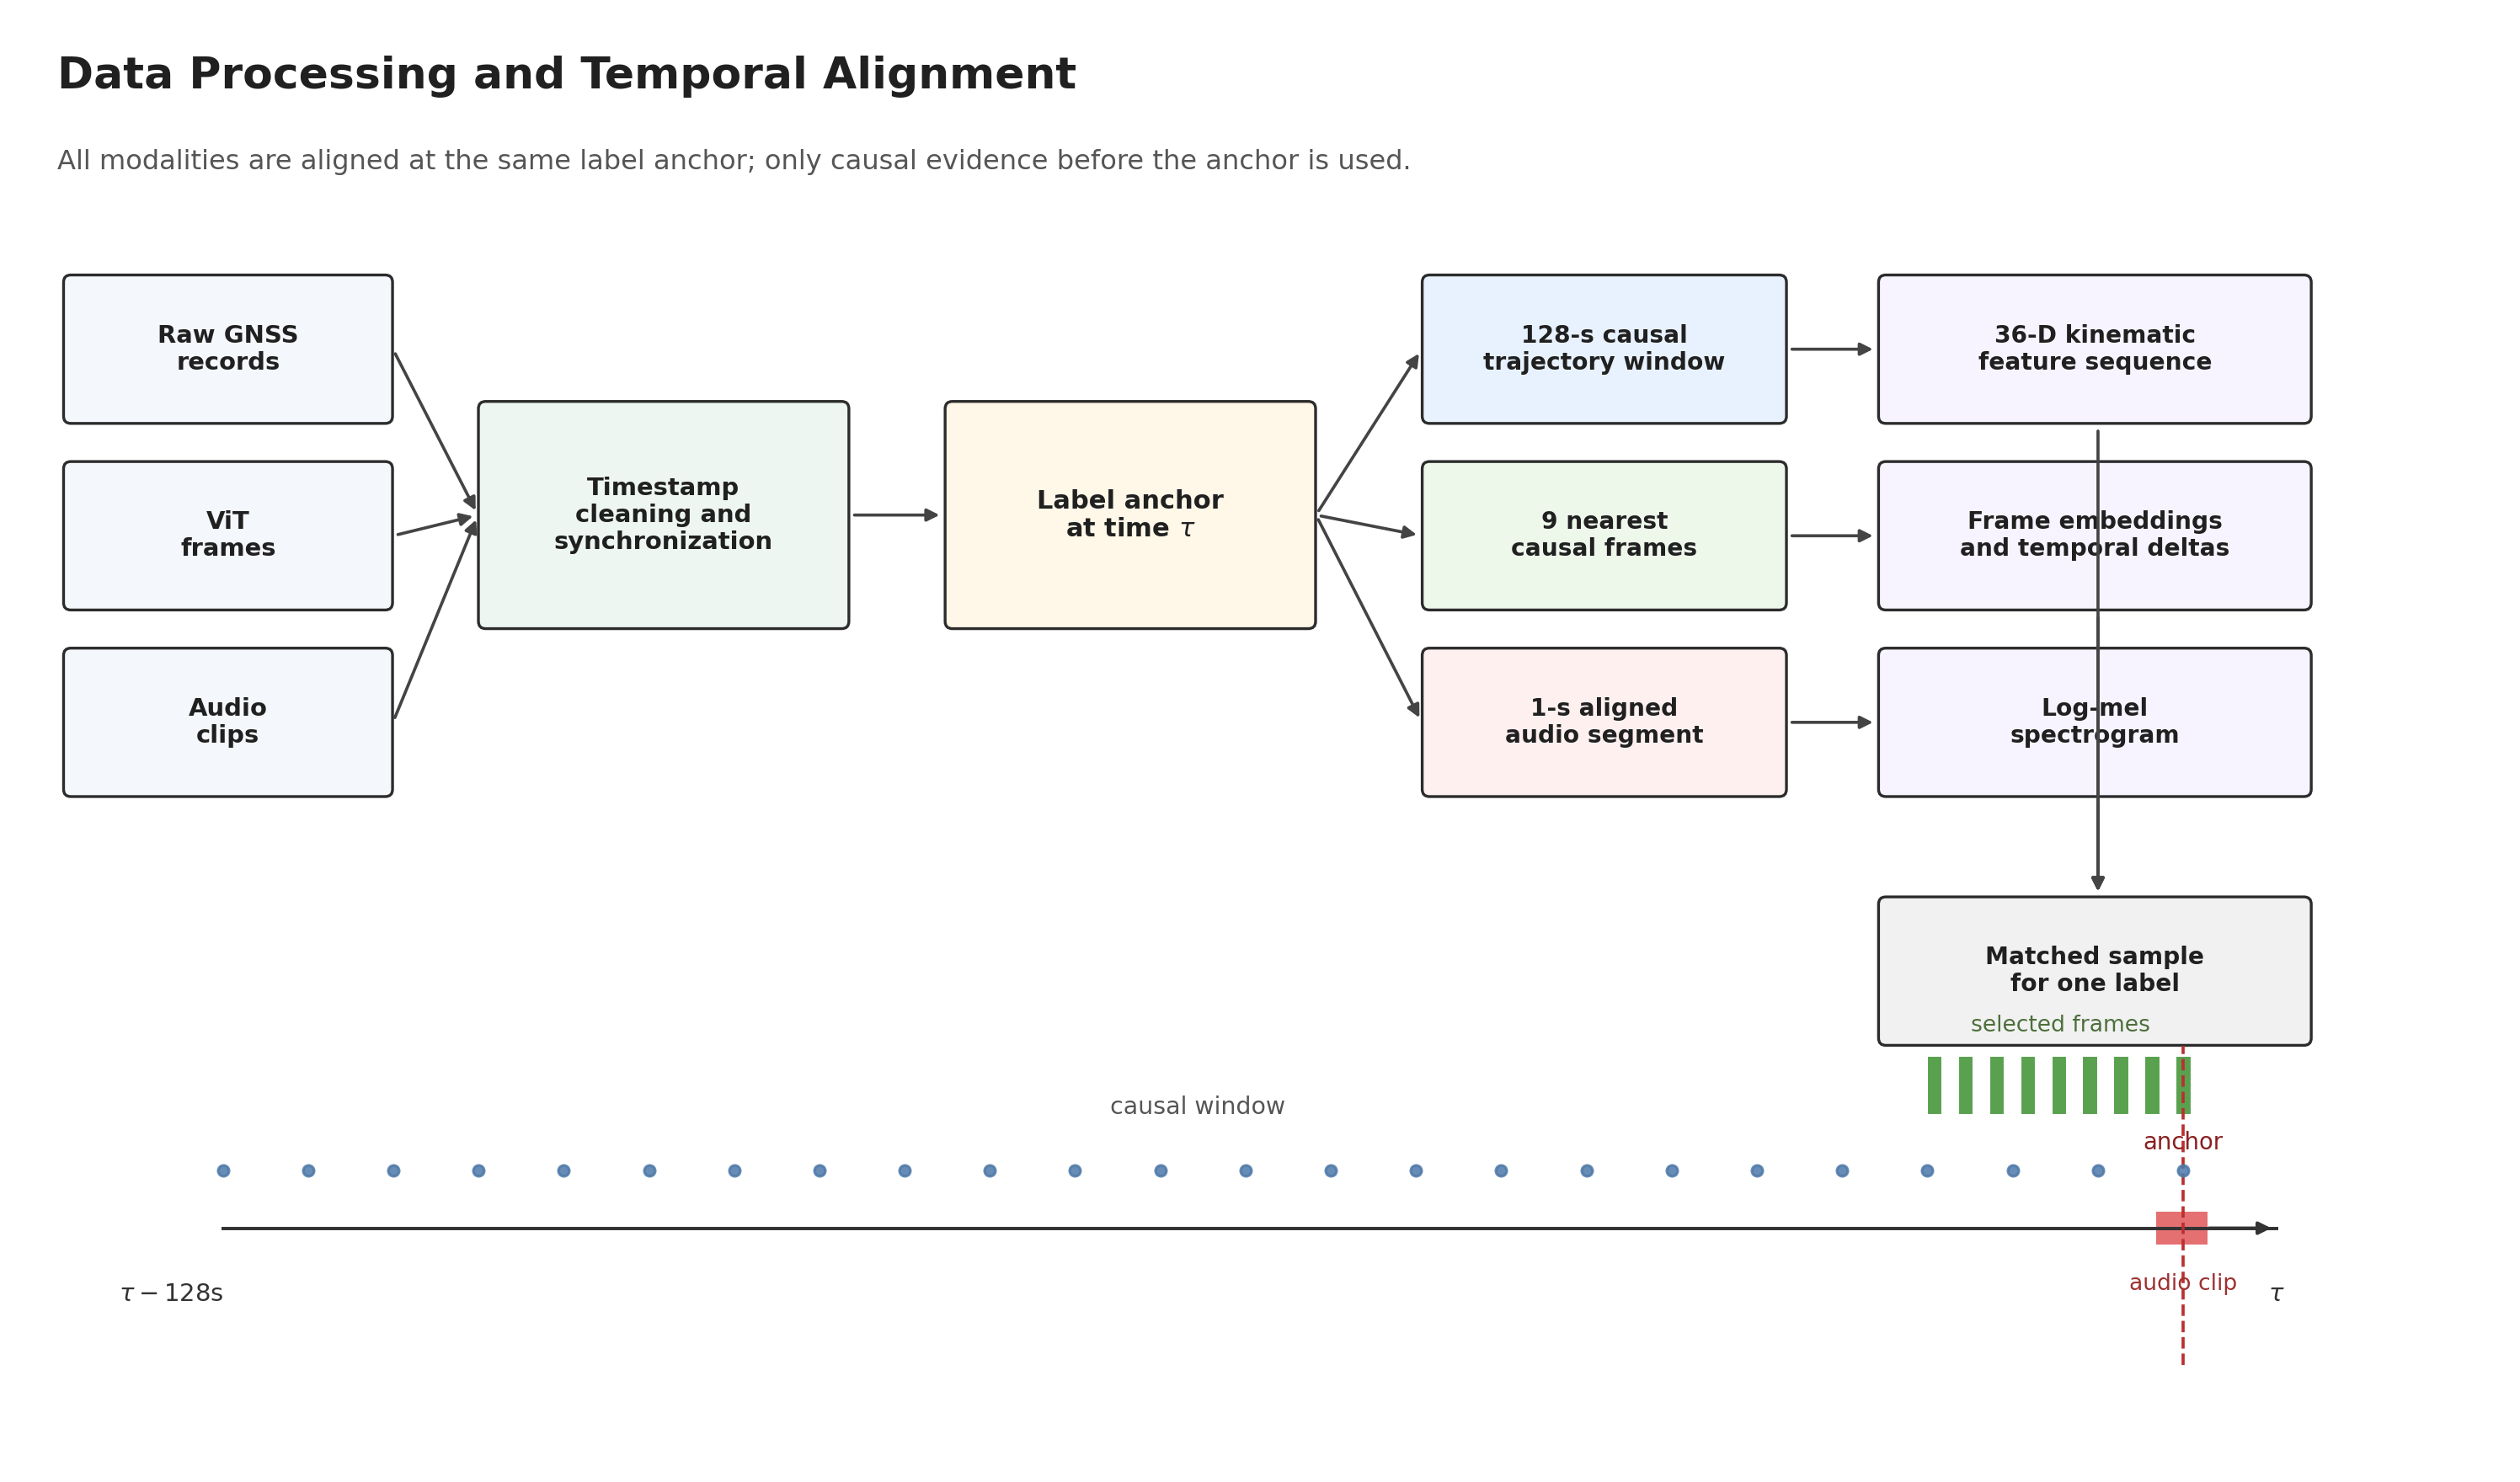
\includegraphics[width=0.98\linewidth]{fig_method_data_processing.png}
\caption{Data processing and temporal alignment workflow. Each label is associated with one anchor time $\tau$. The trajectory branch receives a 128-s causal sequence, the ViT branch receives the nine nearest causal frames from the same window, and the audio branch receives the one-second segment aligned to the anchor. The three processed streams form one matched multimodal sample for classification.}
\label{fig:method_data_processing}
\end{figure}
\FloatBarrier

\subsection{Trajectory Encoder}
\label{sec:trajectory_encoder}

The trajectory branch describes the continuous motion state of the machine before the label time. For each anchor time $\tau$, the input is a causal sequence of $T=128$ one-second samples. A raw trajectory point is denoted as
\begin{equation}
    X_i = (\lambda_i, \phi_i, v_i, d_i, \theta_i, t_i),
\end{equation}
where $\lambda_i$ and $\phi_i$ are longitude and latitude, $v_i$ is speed, $d_i$ is the recorded cutting-depth-related variable, $\theta_i$ is the heading angle, and $t_i$ is the timestamp. These original attributes provide the instantaneous measurement at one point, but they do not fully describe how the machine is moving over a short period. This limitation is important for \task{}, because several operation classes differ mainly in motion evolution. For example, straight harvesting and transfer can share similar speeds, while turning empty harvesting and turning transfer require the model to compare heading, curvature, speed, and working-context changes over time.

We therefore use a multi-view trajectory feature extraction procedure before the neural encoder. It has two causal stages: instantaneous physical feature extraction (IPE) and multi-window statistical extraction (MWSE). IPE converts the original GNSS attributes into interpretable kinematic variables. To avoid artificial discontinuities around $0^\circ/360^\circ$, heading differences are computed with circular wrap-around:
\begin{equation}
    \Delta^{c}\theta_i = ((\theta_i - \theta_{i-1} + 180) \bmod 360) - 180 .
\end{equation}
Let $\Delta t_i=t_i-t_{i-1}$. Since the valid trajectory stream is sampled at 1 Hz inside each contiguous segment, $\Delta t_i=1$ s in normal samples; the formulas below are written in rate form for clarity. The core IPE variables are
\begin{align}
    a_i &= \frac{v_i-v_{i-1}}{\Delta t_i}, \\
    s_i &= v_i-v_{i-1}, \\
    \omega_i &= \frac{\Delta^{c}\theta_i}{\Delta t_i}, \\
    \alpha_i &= \frac{\omega_i-\omega_{i-1}}{\Delta t_i}, \\
    g_i &= \omega_i-\omega_{i-1},
\end{align}
where $a_i$ is acceleration, $s_i$ is speed difference, $\omega_i$ is angular speed, $\alpha_i$ is angular acceleration, and $g_i$ is angular-speed difference. In the implementation, these quantities are computed separately within each contiguous video segment; the first sample of a segment uses zero first-order difference by prepending itself.

Additional IPE descriptors are included to represent spatial displacement, work-state variation, and turning intensity:
\begin{align}
    \Delta \lambda_i &= \lambda_i-\lambda_{i-1}, &
    \Delta \phi_i &= \phi_i-\phi_{i-1}, &
    \Delta d_i &= d_i-d_{i-1}, \\
    j_i &= a_i-a_{i-1}, &
    \kappa_i &= \frac{\omega_i}{|v_i| + 10^{-3}}, &
    e_i &= v_i^2 + |a_i|.
\end{align}
Here $j_i$ is jerk, $\kappa_i$ is a speed-normalized curvature proxy, and $e_i$ is a motion-energy descriptor. The absolute heading change $|\Delta^{c}\theta_i|$ is used as a turning indicator. These instantaneous variables make the trajectory representation sensitive to acceleration, heading transition, local curvature, depth variation, and stop-and-go behavior rather than relying only on raw coordinates and speed.

MWSE then summarizes the recent trajectory context using causal rolling windows. For a scalar IPE series $q_i$, the causal window of length $w$ is
\begin{equation}
    \mathcal{H}_w(i)=\{q_k \mid \max(1,i-w+1) \leq k \leq i\}.
\end{equation}
For $q_i \in \{v_i,a_i,\omega_i,\alpha_i,\Delta^{c}\theta_i\}$ and $w \in \{5,20\}$ seconds, we compute the rolling median and standard deviation:
\begin{equation}
    \operatorname{MWSE}_{5,20}(q_i)=
    [\operatorname{med}(\mathcal{H}_5(i)), \operatorname{med}(\mathcal{H}_{20}(i)),
    \operatorname{std}(\mathcal{H}_5(i)), \operatorname{std}(\mathcal{H}_{20}(i))].
\end{equation}
The 5-s window captures short maneuver changes, while the 20-s window captures more stable operation patterns. We also compute a 3-s local speed mean $\bar{v}^{(3)}_i$ and a 3-s local heading standard deviation $\sigma^{(3)}_{\theta,i}$ from the current and two previous samples. All IPE and MWSE features are causal and therefore use only observations at or before the current time.

The final trajectory feature vector has 36 dimensions:
\begin{equation}
\begin{split}
    \vx_i^t = [&\lambda_i, \phi_i, v_i, a_i, \omega_i, \alpha_i, \Delta^{c}\theta_i, \\
    &\operatorname{MWSE}_{5,20}(v_i,a_i,\omega_i,\alpha_i,\Delta^{c}\theta_i), \\
    &\Delta \lambda_i, \Delta \phi_i, j_i, \kappa_i, e_i, |\Delta^{c}\theta_i|,
    \bar{v}^{(3)}_i, \sigma^{(3)}_{\theta,i}, \Delta d_i].
\end{split}
\end{equation}
The feature construction is performed before sample extraction and is restricted to each contiguous video segment. When a causal 128-s sample extends before the segment beginning, the earliest valid sample is repeated; no observations from other segments or from the future are used. The resulting $\vx^{t}\in\R^{128\times36}$ sequence is normalized using the mean and standard deviation estimated from the training split only.

After feature extraction, the sequence is encoded by a BiLSTM-style neural encoder. Each 36-D vector is reshaped into a $6\times6$ feature map:
\begin{equation}
    M_i=\operatorname{reshape}(\vx_i^t,6,6).
\end{equation}
A point-wise CNN with two convolution--batch-normalization--ReLU blocks and max pooling extracts local interactions among the kinematic variables:
\begin{equation}
    \vp_i = \psi_{\mathrm{cnn}}(M_i).
\end{equation}
The projected point representations $\{\vp_i\}_{i=1}^{128}$ are then passed to a two-layer bidirectional LSTM. The forward and backward states inside the causal window are summed at each time step,
\begin{equation}
    \vh_i = \overrightarrow{\vh}_i + \overleftarrow{\vh}_i,
\end{equation}
and an attention pooling layer aggregates the 128 hidden states into a fixed-dimensional trajectory embedding:
\begin{align}
    \beta_i &= \frac{\exp(\mathbf{w}^{\top}\tanh(\mathbf{W}\vh_i))}
    {\sum_{k=1}^{128}\exp(\mathbf{w}^{\top}\tanh(\mathbf{W}\vh_k))}, \\
    \vz^{t} &= \sum_{i=1}^{128}\beta_i \vh_i = f_t(\vx^{t}).
\end{align}
Although the LSTM is bidirectional within the input sequence, the whole sequence is causal with respect to $\tau$, so the trajectory encoder never uses observations after the label time. This design separates interpretable point-level kinematic construction from sequence-level temporal reasoning. It is especially useful for turning-related and transfer-related behaviors, where the decisive evidence is the recent evolution of heading, curvature, speed, and depth-related variables rather than any single GNSS point.

\subsection{ViT Visual Encoder}

The ViT modality captures visual context such as field texture, crop intake, road surface, and the machine's local working environment. Each selected frame is resized to $224 \times 224$ and encoded by a pretrained ViT-style visual backbone~\cite{dosovitskiy2021vit}. The current best ViT configuration uses nine nearest causal frames, temporal GRU pooling, and frame-difference features. For frame embeddings $\{\vh_i^{v}\}_{i=1}^{9}$, the temporal pooling module produces
\begin{equation}
    \vz^{v} = f_v(\vh_1^{v}, \ldots, \vh_9^{v}).
\end{equation}
This design keeps the visual evidence close to the decision time and avoids using visual frames from the future.

\subsection{Audio Encoder}

The audio modality captures engine load, idling, unloading, and mechanical-component engagement. Audio clips are transformed into log-mel spectrograms and encoded using an Audio Spectrogram Transformer initialized from AudioSet-pretrained weights~\cite{gong2021ast}. The audio encoder outputs
\begin{equation}
    \vz^{a} = f_a(\vx^{a}).
\end{equation}
Audio is expected to be especially useful for distinguishing classes with similar or stationary trajectories, such as engine-off waiting, idling waiting, and unloading.

\subsection{Class-Adaptive Trimodal Fusion}
\label{sec:class_gate}

The proposed trimodal model uses class-adaptive logit fusion instead of direct feature concatenation. This design is motivated by the observation that different operation classes are dominated by different evidence sources. Motion-dependent classes require trajectory curvature, heading change, and speed transitions; scene-dependent classes benefit from ViT visual context; process states such as engine-off waiting, idling waiting, and unloading are often better captured by audio.

For modality $m \in \{t,v,a\}$, a modality-specific classifier head maps the embedding $\vz^m$ to eleven-class logits:
\begin{equation}
    \vl^{m} = q_m(\vz^m), \quad \vl^{m} \in \R^{11}.
\end{equation}
A gating network receives the same three modality embeddings and outputs a class-specific softmax weight $g_{c}^{m}$ over modalities:
\begin{equation}
    \sum_m g_{c}^{m}=1, \quad g_{c}^{m} \geq 0 .
\end{equation}
The final logit for class $c$ is
\begin{equation}
    l_c = \sum_m g_{c}^{m} l_c^{m}.
\end{equation}
The predicted distribution is then
\begin{equation}
    p(y \mid \vx) = \softmax(\vl).
\end{equation}

In the implementation, each modality first passes through layer normalization, dropout, and a lightweight classifier head. The gate projects each modality embedding into a shared gate space, concatenates the three gate features, and predicts an $11 \times 3$ matrix of class-modality weights. The final gate layer is initialized to zero, so the model starts from nearly uniform modality weights and learns class-specific preferences during training. This formulation allows the model to preserve audio-dominant evidence for process classes while assigning more weight to BiLSTM or ViT evidence for motion and scene classes.

The trimodal model is initialized from the unimodal checkpoints for the same seed. The encoders are frozen for the first epoch and then jointly trained, which stabilizes the fusion module while preserving the unimodal representations learned in the preceding runs.

\subsection{Concatenation Reference}

For reference, we also keep a direct concatenation baseline:
\begin{equation}
    \vz = [\vz^{t}; \vz^{v}; \vz^{a}],
\end{equation}
followed by layer normalization, dropout, and a multilayer classifier. This baseline establishes whether the three modalities are complementary under a matched temporal protocol, but it uses one shared classifier for all classes and therefore cannot explicitly preserve class-specific modality dominance.

\subsection{Training Objective and Model Selection}

All models are trained with class-weighted cross-entropy to reduce the dominance of frequent operation classes:
\begin{equation}
    \cL = -\frac{1}{N}\sum_{i=1}^{N} w_{y_i}\log p(y_i \mid \vx_i),
\end{equation}
where $w_{y_i}$ is derived from the inverse class frequency with a power coefficient. The main selection metric is validation macro-F1:
\begin{equation}
    \mathrm{MacroF1} = \frac{1}{11}\sum_{c=0}^{10} \mathrm{F1}_{c}.
\end{equation}
Macro-F1 weights every class equally and is therefore more appropriate than accuracy for this imbalanced eleven-class problem. A checkpoint is saved only when validation macro-F1 improves by more than the early-stopping threshold.

\section{Experiments}
\label{sec:exp}

\subsection{Dataset and Annotation}

The experiments use synchronized data collected from real combine-harvester operations during three months of maize harvesting in Ningxia, Shaanxi, and Inner Mongolia. Each timestamped record is associated with GNSS trajectory measurements, image frames, audio, and an eleven-class operation label. The current paper suite uses the cleaned multimodal split stored as \texttt{data/b\_deep\_part\_multimodal\_full\_clean\_20260417}. The split contains 114,628 training rows, 33,078 validation rows, and 36,447 test rows. Under the adaptive causal-window sampler, the training split yields 53,936 training windows for \texttt{seq\_len}=128. Validation and test use dense evaluation with stride 1, so every labeled timestamp is evaluated.

The multimodal subset is selected to emphasize the characteristics that cannot be studied in an audio-only setting. Each retained sample must have a valid trajectory record, a synchronized ViT visual observation, and an available audio segment; only four training rows are filled with silence, while all validation and test rows contain real audio. This selection produces a larger and more diverse benchmark than the earlier audio-only setting, while ensuring that the comparison among trajectory, ViT, audio, and trimodal models is made on exactly the same samples. \Cref{fig:dataset_distribution} summarizes the absolute class counts and the split-wise class proportions. Final numerical results are reported on the full held-out test set rather than on selected cases.

\begin{figure}[t]
\centering
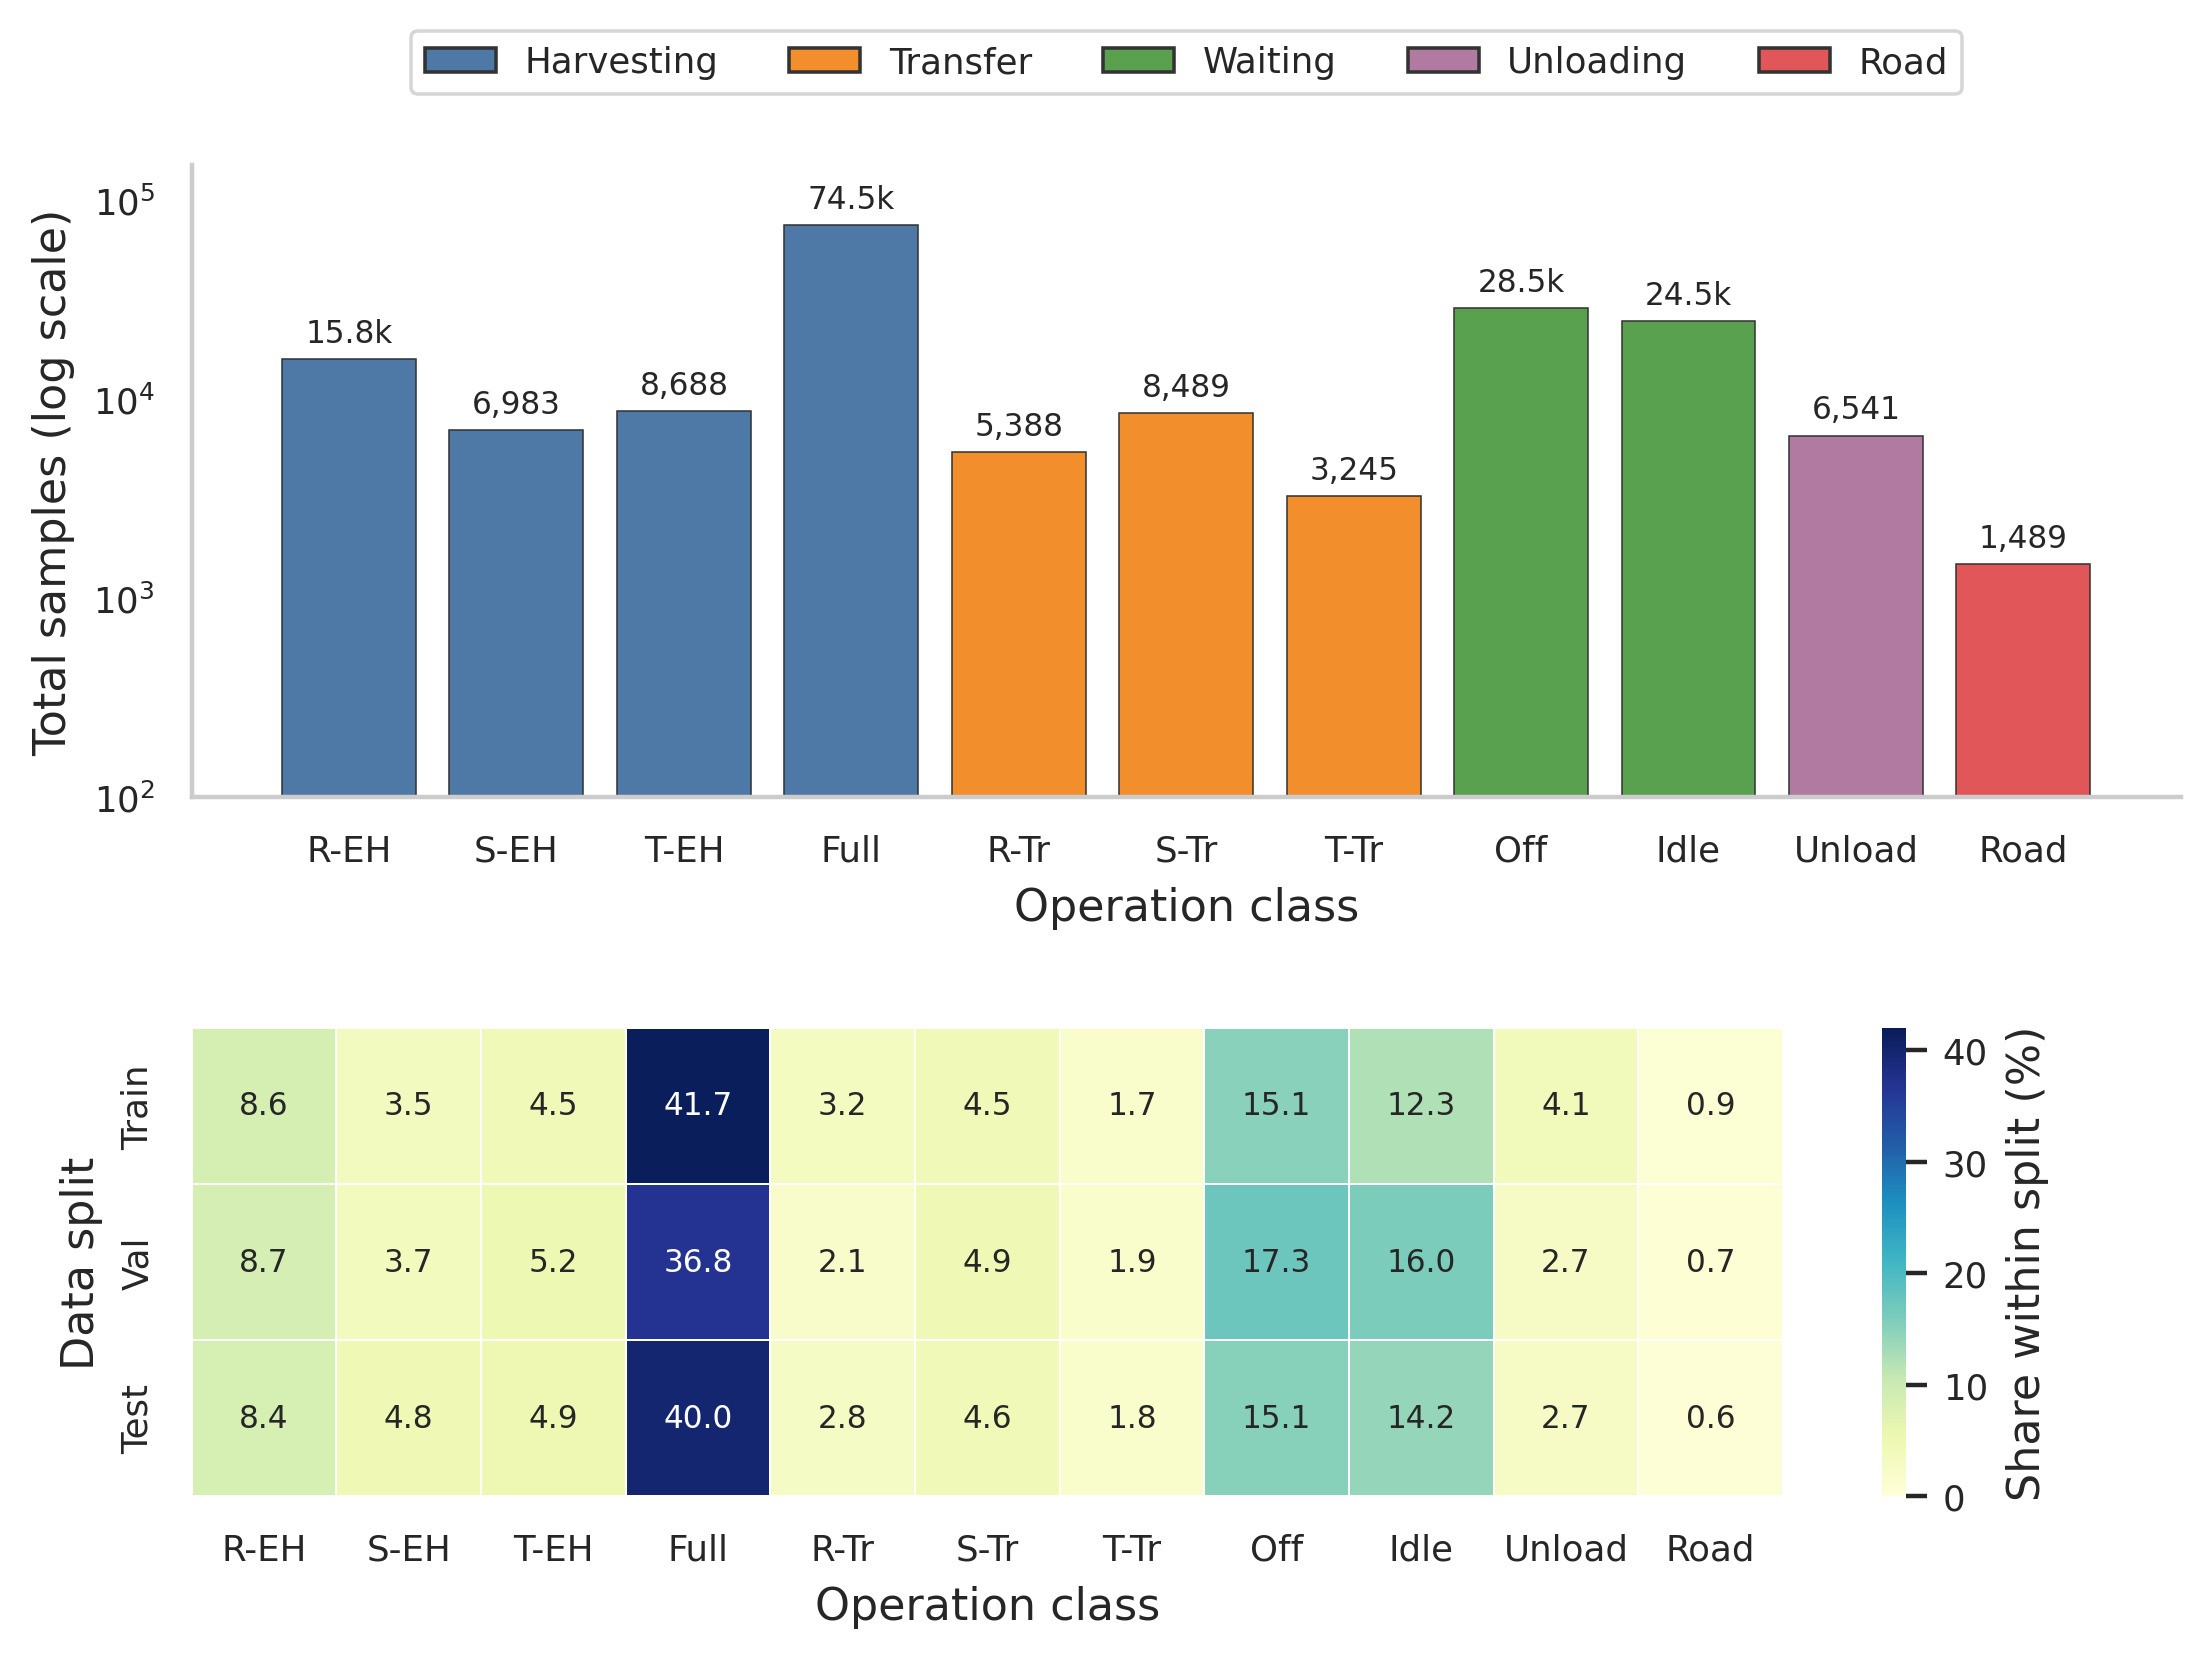
\includegraphics[width=0.92\linewidth]{fig_dataset_distribution.png}
\caption{Class distribution of the cleaned multimodal split. The upper panel reports total samples per class on a logarithmic scale, with colors indicating operation groups. The lower panel reports the percentage of each class within the training, validation, and test splits. The distribution reflects naturally imbalanced agricultural operations: full-load harvesting and waiting states dominate the corpus, whereas turning transfer and road driving are minority classes.}
\label{fig:dataset_distribution}
\end{figure}
\FloatBarrier

\subsection{Class Taxonomy}

The label space contains eleven operation categories covering harvesting, transfer, waiting, unloading, and road driving. \Cref{tab:classes} lists the unified taxonomy used throughout this paper. The dominant-evidence column summarizes the empirical behavior observed in the current fixed-seed suite.

\begin{table}[t]
\centering
\caption{Eleven classes for \task{}.}
\label{tab:classes}
\small
\begin{tabular}{clll}
\toprule
\textbf{ID} & \textbf{Class} & \textbf{Group} & \textbf{Dominant evidence} \\
\midrule
0  & Reverse empty harvesting  & Harvesting & ViT + trajectory \\
1  & Straight empty harvesting & Harvesting & ViT + multimodal context \\
2  & Turning empty harvesting  & Harvesting & ViT + trajectory \\
3  & Full-load harvesting      & Harvesting & audio + ViT \\
4  & Reverse transfer          & Transfer   & trajectory + ViT \\
5  & Straight transfer         & Transfer   & trajectory + audio \\
6  & Turning transfer          & Transfer   & trajectory + ViT; rare, ambiguous \\
7  & Engine-off waiting        & Waiting    & audio \\
8  & Idling waiting            & Waiting    & audio \\
9  & Unloading                 & Unloading  & audio \\
10 & Road driving              & Road       & ViT + trajectory \\
\bottomrule
\end{tabular}
\end{table}

This taxonomy intentionally includes classes that are difficult for a single modality. Waiting and unloading classes are often spatially overlapping; empty harvesting and transfer classes can share similar motion; and full-load harvesting is visually and acoustically different from other harvesting states but can still follow similar field paths.

\subsection{Implementation Details}

The final paper suite, \texttt{paper\_4090\_final\_seed44}, is run on three NVIDIA RTX 4090 GPUs with physical IDs 1, 2, and 5. All final-suite models use a fixed seed of 44, selected from the best BiLSTM trajectory run in the completed sequence-length ablation. The shared causal trajectory length is 128 seconds. ViT experiments use nine nearest causal frames within the same 128-second window, and audio uses the one-second waveform segment aligned to the anchor time. The batch size is 48 for BiLSTM, ViT, and AST experiments, and 24 for trimodal fusion. Early stopping monitors validation macro-F1 with \texttt{min\_delta}=0.001. BiLSTM, ViT, and AST are trained for up to 20 epochs with patience 6; trimodal models are trained for up to 24 epochs with patience 8.

\subsection{Multimodal Experimental Design}
\label{sec:multimodal_design}

The multimodal experiments are designed to test whether synchronized motion, scene, and process cues are complementary under the same temporal protocol. In the codebase, \texttt{multimodal} denotes the trajectory--ViT setting, whereas \texttt{trimodal} denotes trajectory--ViT--audio. The paper focuses on the trimodal setting because the target taxonomy contains classes that cannot be reliably separated by a single evidence source.

The experimental protocol has three stages. First, we train three unimodal baselines on the same split and with the same anchor times: BiLSTM for trajectory, the ViT-GRU model for visual frames, and AST for audio. These baselines quantify the independent contribution of each modality. Second, we initialize the trimodal model from the three corresponding unimodal checkpoints. The encoders are frozen for one warmup epoch so that the fusion module can adapt to the scale of the pretrained modality embeddings. After the warmup epoch, all branches are jointly optimized with a smaller learning rate. Third, we evaluate the proposed class-adaptive fusion strategy against a direct concatenation reference.

The proposed fusion experiment is \texttt{trimodal\_class\_gate}. It uses the class-adaptive logit fusion described in \Cref{sec:class_gate}. Each modality first predicts its own eleven-class logits, and a gating network learns class-specific modality weights. This design directly targets the modality imbalance observed in the completed baselines: AST is strongest for stationary process states, whereas BiLSTM and ViT cues are more informative for turning, transfer, road driving, and harvesting-context classes.

The direct concatenation reference is \texttt{trimodal\_concat}. It concatenates the BiLSTM embedding, the ViT embedding, and the AST embedding, followed by layer normalization, dropout, and a multilayer classifier. This model answers the basic question of whether the three modalities provide complementary information when combined with a simple and reproducible fusion rule, but it does not explicitly assign different modality weights to different classes.

The main comparison is reported at three levels. At the aggregate level, we compare accuracy, macro-F1, and weighted-F1 against the best unimodal baseline. At the class level, we compare per-class F1 and recall to identify which behaviors benefit from fusion and which remain better handled by a single modality. At the diagnostic level, we inspect complete held-out trajectory parts to determine whether the same gains are visible on continuous field trajectories. Particular attention is paid to turning empty harvesting and turning transfer, because these classes require temporal motion evidence from trajectory and harvesting-context evidence from ViT or audio rather than a single-frame visual cue.

\subsection{Evaluation Metrics}

We report accuracy, macro-F1, weighted-F1, per-class recall, confusion matrices, and trajectory-level diagnostic plots. Macro-F1 is the main model-selection metric because the class distribution is strongly imbalanced. A high accuracy can be obtained by favoring frequent classes such as full-load harvesting, whereas macro-F1 penalizes failure on minority classes such as turning transfer and road driving.

\subsection{Sequence-Length Ablation for BiLSTM}
\label{sec:seq_ablation}

Before launching the final multimodal suite, we evaluated BiLSTM with sequence lengths of 64, 128, 256, and 512 seconds across four seeds. \Cref{tab:seq_len} summarizes the completed ablation.

\begin{table}[t]
\centering
\caption{BiLSTM sequence-length ablation across seeds 42--45. Values are mean $\pm$ standard deviation.}
\label{tab:seq_len}
\small
\begin{tabular}{lccc}
\toprule
\textbf{Sequence length} & \textbf{Accuracy} & \textbf{Macro-F1} & \textbf{Weighted-F1} \\
\midrule
64 s  & $0.7232 \pm 0.0055$ & $0.5273 \pm 0.0055$ & $0.7202 \pm 0.0034$ \\
128 s & $\mathbf{0.7308 \pm 0.0130}$ & $\mathbf{0.5464 \pm 0.0135}$ & $\mathbf{0.7282 \pm 0.0098}$ \\
256 s & $0.7240 \pm 0.0125$ & $0.5385 \pm 0.0120$ & $0.7255 \pm 0.0108$ \\
512 s & $0.6890 \pm 0.0309$ & $0.5190 \pm 0.0190$ & $0.6944 \pm 0.0267$ \\
\bottomrule
\end{tabular}
\end{table}

The best mean macro-F1 is obtained at 128 seconds. The best single run is also \texttt{seq\_len}=128 with seed 44, achieving 73.72\% accuracy, 56.05\% macro-F1, and 73.38\% weighted-F1. The 512-second setting has larger variance and lower test performance, suggesting that long causal windows introduce stale context and optimization noise. The 64-second setting is stable but misses longer transition information. Therefore, all final paper experiments use \texttt{seq\_len}=128.

\subsection{Final Fixed-Seed Results}
\label{sec:final_results}

\Cref{tab:paper_suite} reports the completed fixed-seed results. Direct trimodal concatenation already improves over all single-modality baselines, reaching 79.16\% accuracy, 61.19\% macro-F1, and 78.44\% weighted-F1. The proposed class-adaptive fusion model uses the same seed, split, temporal protocol, unimodal initialization, and batch size, but replaces the single concatenated classifier with class-wise logit gating. It reaches 81.36\% accuracy, 63.64\% macro-F1, and 81.01\% weighted-F1. Compared with direct concatenation, this is an improvement of 2.21 accuracy points, 2.44 macro-F1 points, and 2.56 weighted-F1 points. Compared with BiLSTM, the strongest single-modality baseline by macro-F1, \ours{} improves macro-F1 by 9.00 points.

\begin{table}[t]
\centering
\caption{Fixed-seed test results and fusion ablation. All trimodal models use the same unimodal initialization and temporal protocol. Values are reported in percent.}
\label{tab:paper_suite}
\small
\resizebox{\linewidth}{!}{%
\begin{tabular}{llcccc}
\toprule
\textbf{Model} & \textbf{Input} & \textbf{Batch} & \textbf{Accuracy} & \textbf{Macro-F1} & \textbf{Weighted-F1} \\
\midrule
AST & audio spectrogram & 48 & 74.24 & 46.57 & 72.85 \\
ViT & nine causal frames & 48 & 69.49 & 51.96 & 69.53 \\
BiLSTM & trajectory & 48 & 73.37 & 54.63 & 73.47 \\
TIM concat & trajectory + ViT + audio & 24 & 79.16 & 61.19 & 78.44 \\
\textbf{\ours{} class-gate} & trajectory + ViT + audio & 24 & \textbf{81.36} & \textbf{63.64} & \textbf{81.01} \\
\bottomrule
\end{tabular}
}
\end{table}

The single-modality results show different strengths. BiLSTM is the most balanced unimodal model and performs well on motion-dependent transfer classes. ViT-only classification is useful for visually grounded classes, especially empty harvesting and road driving, but it overfits strongly: training macro-F1 reaches 97.23\% by epoch 20 while the selected validation macro-F1 is 54.47\%. AST is highly effective on process-dominated classes but weak on many minority motion classes, which explains the gap between its accuracy and macro-F1. The class-adaptive fusion result shows that the gain is not only from adding modalities, but also from changing how the modalities are combined.

\begin{figure}[t]
\centering
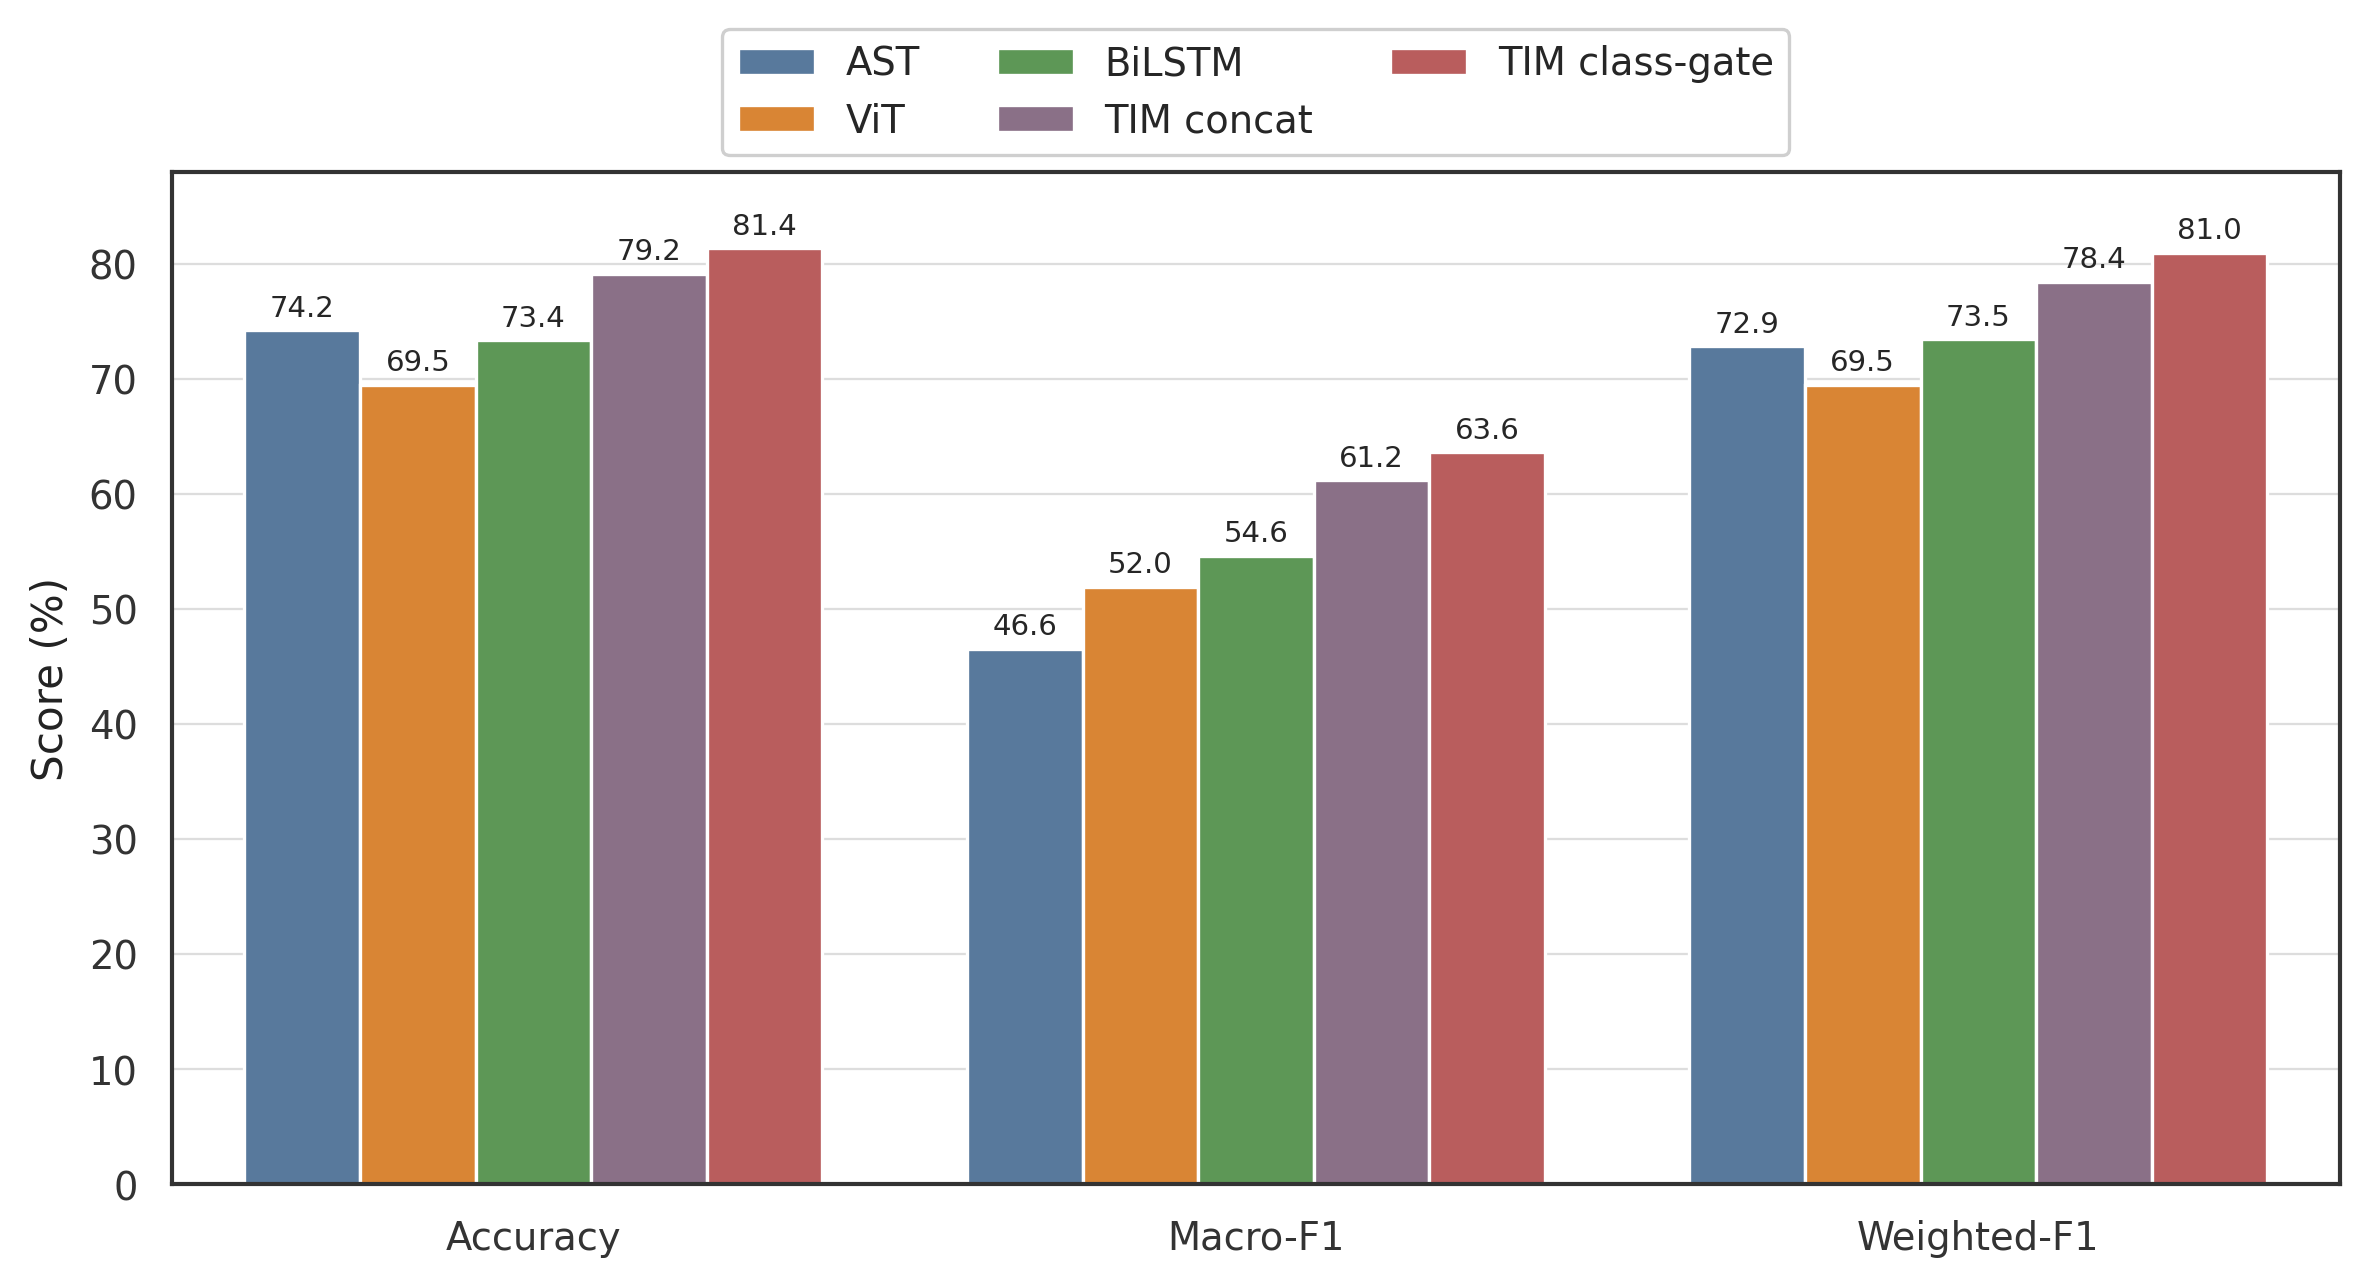
\includegraphics[width=0.82\linewidth]{fig_overall_results.png}
\caption{Overall fixed-seed performance of unimodal baselines, direct trimodal concatenation, and the proposed class-adaptive gate. The class-gate fusion model gives the best accuracy, macro-F1, and weighted-F1 under the same test split.}
\label{fig:overall_results}
\end{figure}
\FloatBarrier

\subsection{Fusion Module Ablation}
\label{sec:fusion_ablation}

\Cref{fig:fusion_ablation} summarizes the direct comparison between \texttt{trimodal\_concat} and \texttt{trimodal\_class\_gate}. The selected case-study data are chosen by a fixed diagnostic rule: we use the same held-out trajectory parts as the modality diagnostics and report every selected part, while the error-pair panel lists the largest reductions in wrong true--predicted pairs when replacing concatenation with the class gate. This selection highlights the improvements without hiding the one trajectory where concatenation remains slightly better.

The class gate improves seven of the eleven per-class F1 scores relative to concatenation. The largest gains occur for turning transfer (+11.74 F1 points), idling waiting (+9.60), reverse transfer (+5.59), engine-off waiting (+4.73), and turning empty harvesting (+4.45). These classes are exactly where the evidence source changes by class: turning transfer needs motion and scene context, while waiting states depend strongly on audio. At the error-pair level, the largest reduction is idling waiting predicted as engine-off waiting, which decreases from 1,564 samples to 773 samples. Other large reductions include straight transfer predicted as reverse transfer (244 to 80), turning empty harvesting predicted as straight empty harvesting (396 to 254), and turning transfer predicted as reverse transfer (230 to 93). On continuous trajectory diagnostics, class-gate fusion is better than concatenation on three of the four selected parts and improves the weighted part-level accuracy from 79.16\% to 81.36\%.

The ablation also identifies the remaining weaknesses. Straight empty harvesting, unloading, and road driving decrease relative to concatenation. In particular, unloading remains better captured by AST than by either trimodal fusion variant, and road driving remains sensitive to the small number of road samples. These results suggest that class-adaptive gating is a useful fusion module, but the gate should be further constrained or regularized for rare scene-dominated and audio-dominated classes.

\begin{figure}[t]
\centering
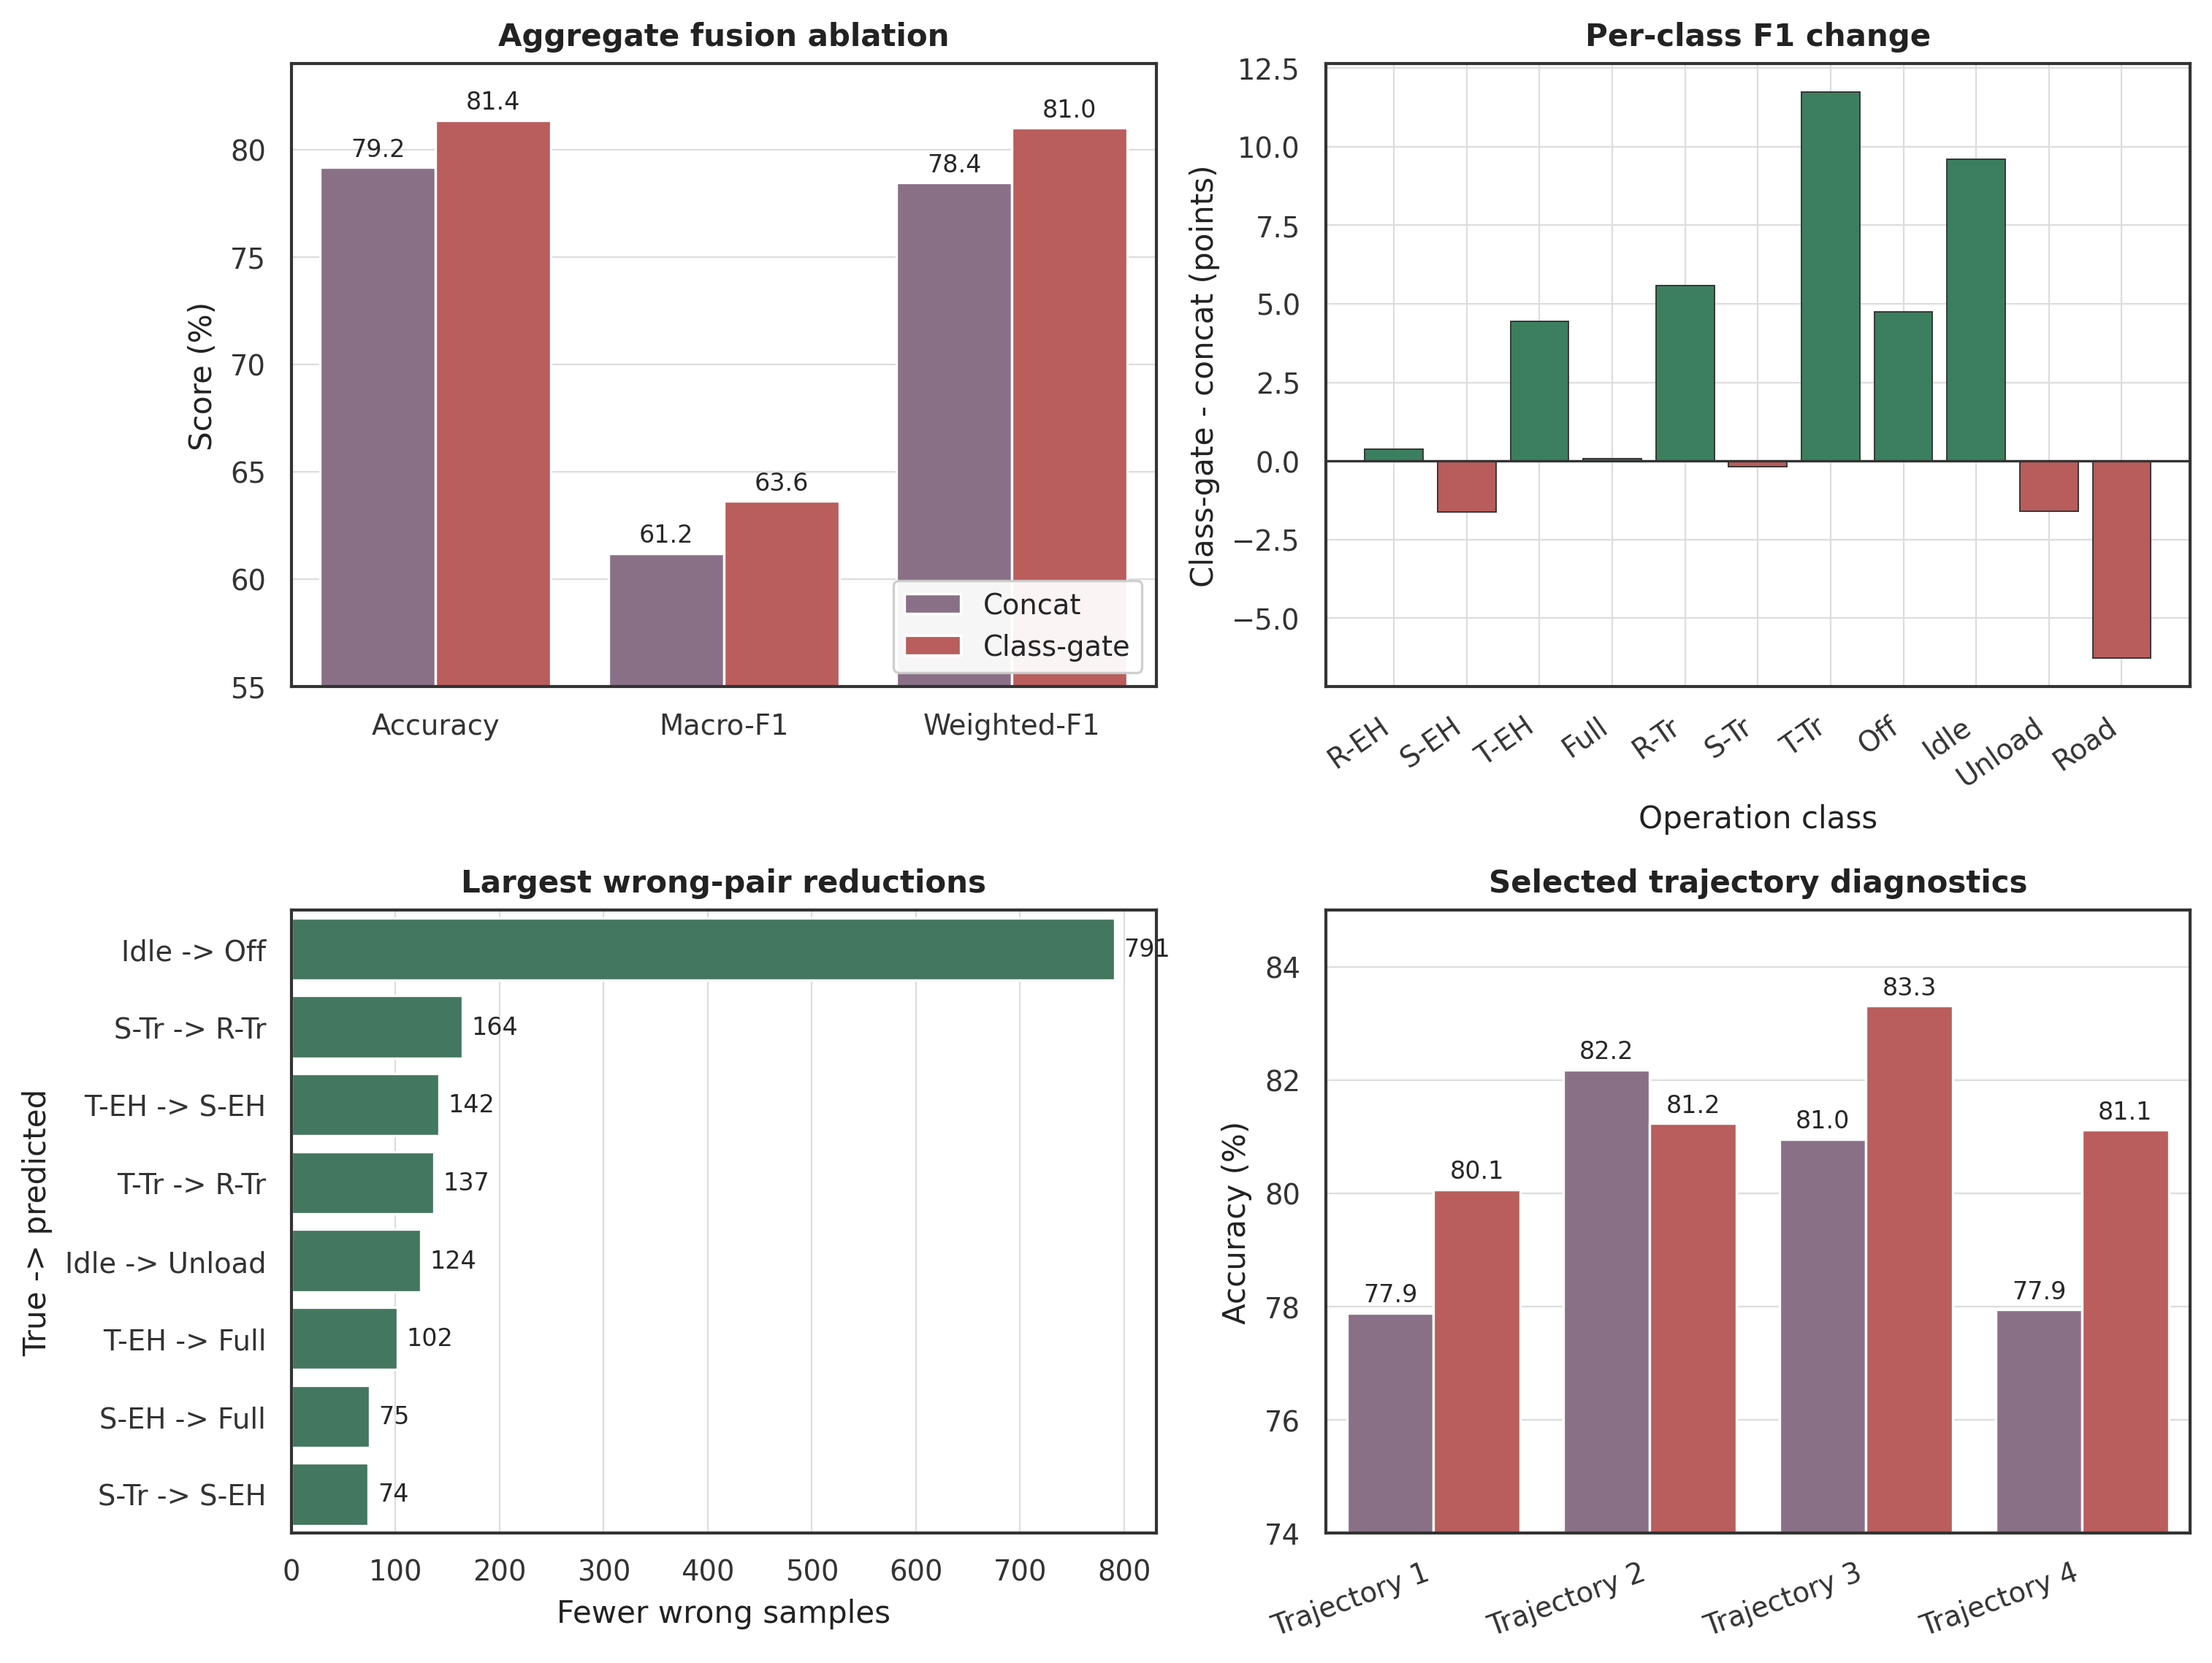
\includegraphics[width=0.98\linewidth]{fig_fusion_ablation.png}
\caption{Fusion module ablation between direct trimodal concatenation and the proposed class-adaptive gate. The panels report aggregate test metrics, per-class F1 changes, the largest reductions in wrong true--predicted pairs, and selected trajectory-level accuracies. The selected trajectories are the same held-out diagnostic parts used elsewhere in the paper; all full-test numerical conclusions use the complete test set.}
\label{fig:fusion_ablation}
\end{figure}
\FloatBarrier

\subsection{Per-Class Modality Roles}
\label{sec:modality_roles}

\Cref{tab:per_class_roles} compares the best single modality, direct trimodal concatenation, and the proposed class gate for each class. \ours{} improves over the best single modality on 8 of 11 classes. The largest gains over the best single modality appear in turning transfer, reverse transfer, straight empty harvesting, idling waiting, and turning empty harvesting. The comparison with concatenation shows where the class-adaptive gate is useful: it increases turning transfer from 25.87\% to 37.61\% F1 and idling waiting from 63.56\% to 73.16\% F1.

\begin{table}[t]
\centering
\caption{Per-class comparison among the best single modality, direct trimodal concatenation, and \ours{} class-gate fusion. F1 values are reported in percent.}
\label{tab:per_class_roles}
\scriptsize
\resizebox{\linewidth}{!}{%
\begin{tabular}{clccccc}
\toprule
\textbf{ID} & \textbf{Class} & \textbf{Best single} & \textbf{Concat} & \textbf{Class-gate} & \textbf{$\Delta$ gate-concat} & \textbf{$\Delta$ gate-best} \\
\midrule
0  & Reverse empty harvesting  & ViT 78.11 & 82.60 & 82.97 & +0.38 & +4.86 \\
1  & Straight empty harvesting & ViT 37.46 & 45.30 & 43.67 & -1.63 & +6.21 \\
2  & Turning empty harvesting  & ViT 58.86 & 59.77 & 64.22 & +4.45 & +5.35 \\
3  & Full-load harvesting      & AST 94.78 & 95.66 & 95.72 & +0.06 & +0.94 \\
4  & Reverse transfer          & BiLSTM 53.12 & 61.05 & 66.64 & +5.59 & +13.52 \\
5  & Straight transfer         & BiLSTM 55.41 & 61.08 & 60.91 & -0.18 & +5.50 \\
6  & Turning transfer          & ViT 23.14 & 25.87 & 37.61 & +11.74 & +14.47 \\
7  & Engine-off waiting        & AST 90.08 & 83.63 & 88.36 & +4.73 & -1.72 \\
8  & Idling waiting            & AST 67.05 & 63.56 & 73.16 & +9.60 & +6.11 \\
9  & Unloading                 & AST 42.64 & 40.73 & 39.13 & -1.59 & -3.50 \\
10 & Road driving              & ViT 50.53 & 53.90 & 47.62 & -6.28 & -2.91 \\
\bottomrule
\end{tabular}
}
\end{table}

These results support the intended multimodal interpretation. BiLSTM is most useful for spatial continuity, direction, and transfer motion. ViT is most useful for visible scene context, crop contact, harvesting conditions, and road surface. AST is most useful for engine response, load variation, working-component engagement, and stationary process states. The class gate improves the balance between these evidence sources, especially for idling waiting and turning transfer. However, engine-off waiting remains slightly better for AST alone, and unloading and road driving remain below their best single-modality baselines.

\begin{figure}[t]
\centering
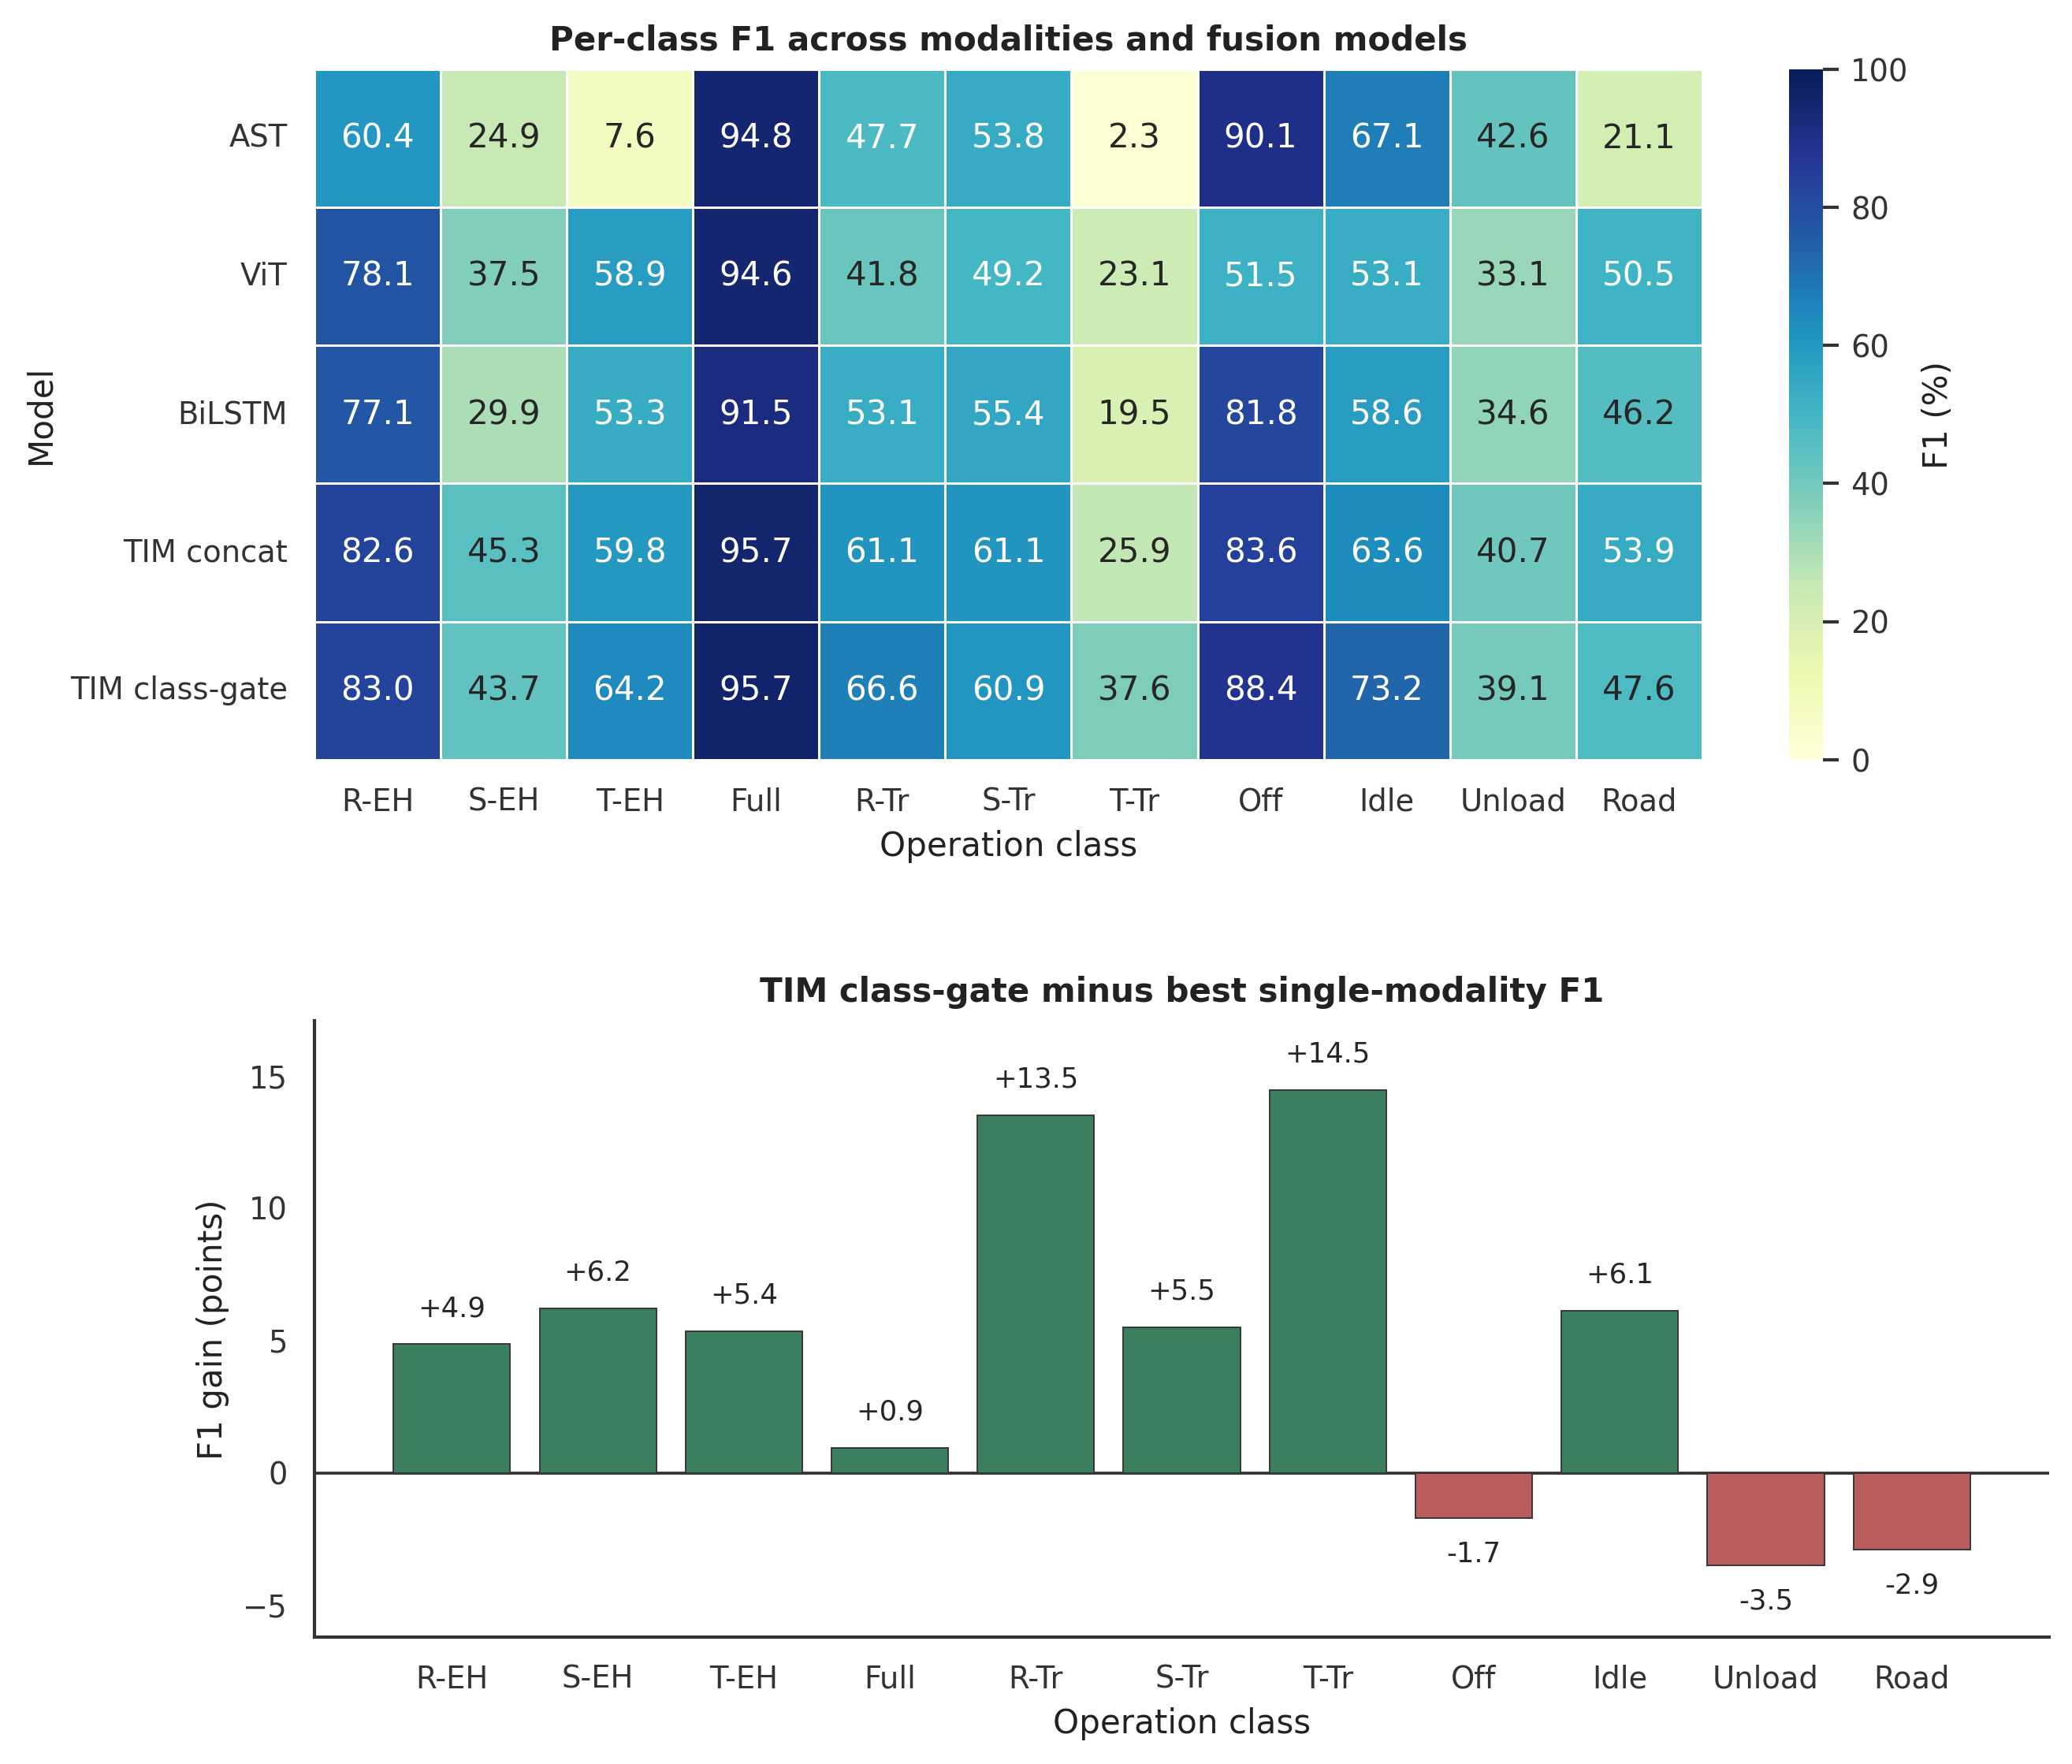
\includegraphics[width=0.98\linewidth]{fig_modality_roles.png}
\caption{Per-class modality roles. The upper panel reports F1 scores for each model and class, while the lower panel shows the F1 difference between \ours{} class-gate fusion and the best single-modality model. Positive bars indicate classes improved by multimodal fusion; negative bars indicate classes where a single modality remains stronger.}
\label{fig:modality_roles}
\end{figure}
\FloatBarrier

\subsection{Error Analysis}
\label{sec:error_analysis}

The weakest \ours{} class is turning transfer, with 37.61\% F1 and 34.98\% recall on 666 test samples. Although this remains a difficult minority class, it is substantially better than direct concatenation, which obtains only 25.87\% F1 and 20.12\% recall. The remaining turning-transfer errors are mainly confused with straight transfer and reverse transfer, indicating that the model often recognizes the transfer group but still fails to separate the turning substate. Unloading is the second major weakness: \ours{} obtains 39.13\% F1 and 33.16\% recall, below the AST-only F1 of 42.64\%. This confirms that unloading is still an audio-dominant process state.

The top remaining \ours{} error pairs are idling waiting $\rightarrow$ engine-off waiting, straight empty harvesting $\rightarrow$ turning empty harvesting, unloading $\rightarrow$ idling waiting, turning transfer $\rightarrow$ straight transfer, full-load harvesting $\rightarrow$ straight empty harvesting, and turning empty harvesting $\rightarrow$ straight empty harvesting. Compared with concatenation, the class gate reduces the largest idling waiting $\rightarrow$ engine-off waiting error from 1,564 to 773 samples, but it increases engine-off waiting $\rightarrow$ idling waiting from 63 to 204 samples. This structure suggests two design requirements: transition-aware temporal modeling for neighboring subactions and gate regularization that can preserve audio dominance for process states without overcorrecting between similar waiting labels.

\subsection{Trajectory-Level Diagnostic Analysis}

In addition to aggregate metrics, we generate trajectory-level diagnostics on complete field parts. These figures plot correct and incorrect predictions over local field coordinates, confusion matrices, dominant misclassification pairs, and class-distribution comparisons. The diagnostics use generic labels such as ``Trajectory 1'' so that they can be inserted into the paper without file-specific naming. For compact case-study figures, we select representative trajectories or intervals using a fixed criterion: the selected case must have sufficient samples and at least two active classes, and it is ranked by the improvement of the trimodal model over the best single-modality model. This selection is used only for visualization; all numerical conclusions remain based on the full held-out test set.

\Cref{tab:part_diag} summarizes the selected part-level accuracies. Direct concatenation already improves over the unimodal baselines on the selected continuous trajectories. The class-adaptive gate further improves three of the four selected parts and gives the best weighted part-level accuracy over all 36,447 diagnostic samples.

\begin{table}[t]
\centering
\caption{Part-level diagnostic accuracy in percent.}
\label{tab:part_diag}
\small
\begin{tabular}{llccccc}
\toprule
\textbf{Trajectory} & \textbf{Part} & \textbf{AST} & \textbf{ViT} & \textbf{BiLSTM} & \textbf{Concat} & \textbf{Class-gate} \\
\midrule
Trajectory 1 & 1 & 68.91 & 72.09 & 70.14 & 77.89 & \textbf{80.07} \\
Trajectory 2 & 2 & 72.27 & 61.23 & 78.35 & \textbf{82.18} & 81.23 \\
Trajectory 3 & 3 & 75.70 & 60.01 & 74.27 & 80.96 & \textbf{83.31} \\
Trajectory 4 & 1 & 75.86 & 74.55 & 72.39 & 77.95 & \textbf{81.12} \\
\bottomrule
\end{tabular}
\end{table}

To make fuller use of the generated diagnostic artifacts, we further aggregate the four held-out trajectory parts. \Cref{fig:part_confusion_modalities} compares part-level confusion matrices for AST, ViT, BiLSTM, TIM concat, and TIM class-gate under the same selected trajectories. The matrix structure is consistent with the full-test results: AST is strong on process states such as full-load harvesting and waiting, ViT helps with visible harvesting and road context, BiLSTM improves motion-related transfer states, and TIM class-gate produces the most balanced part-level diagonal among these reference models.

\begin{figure}[p]
\centering
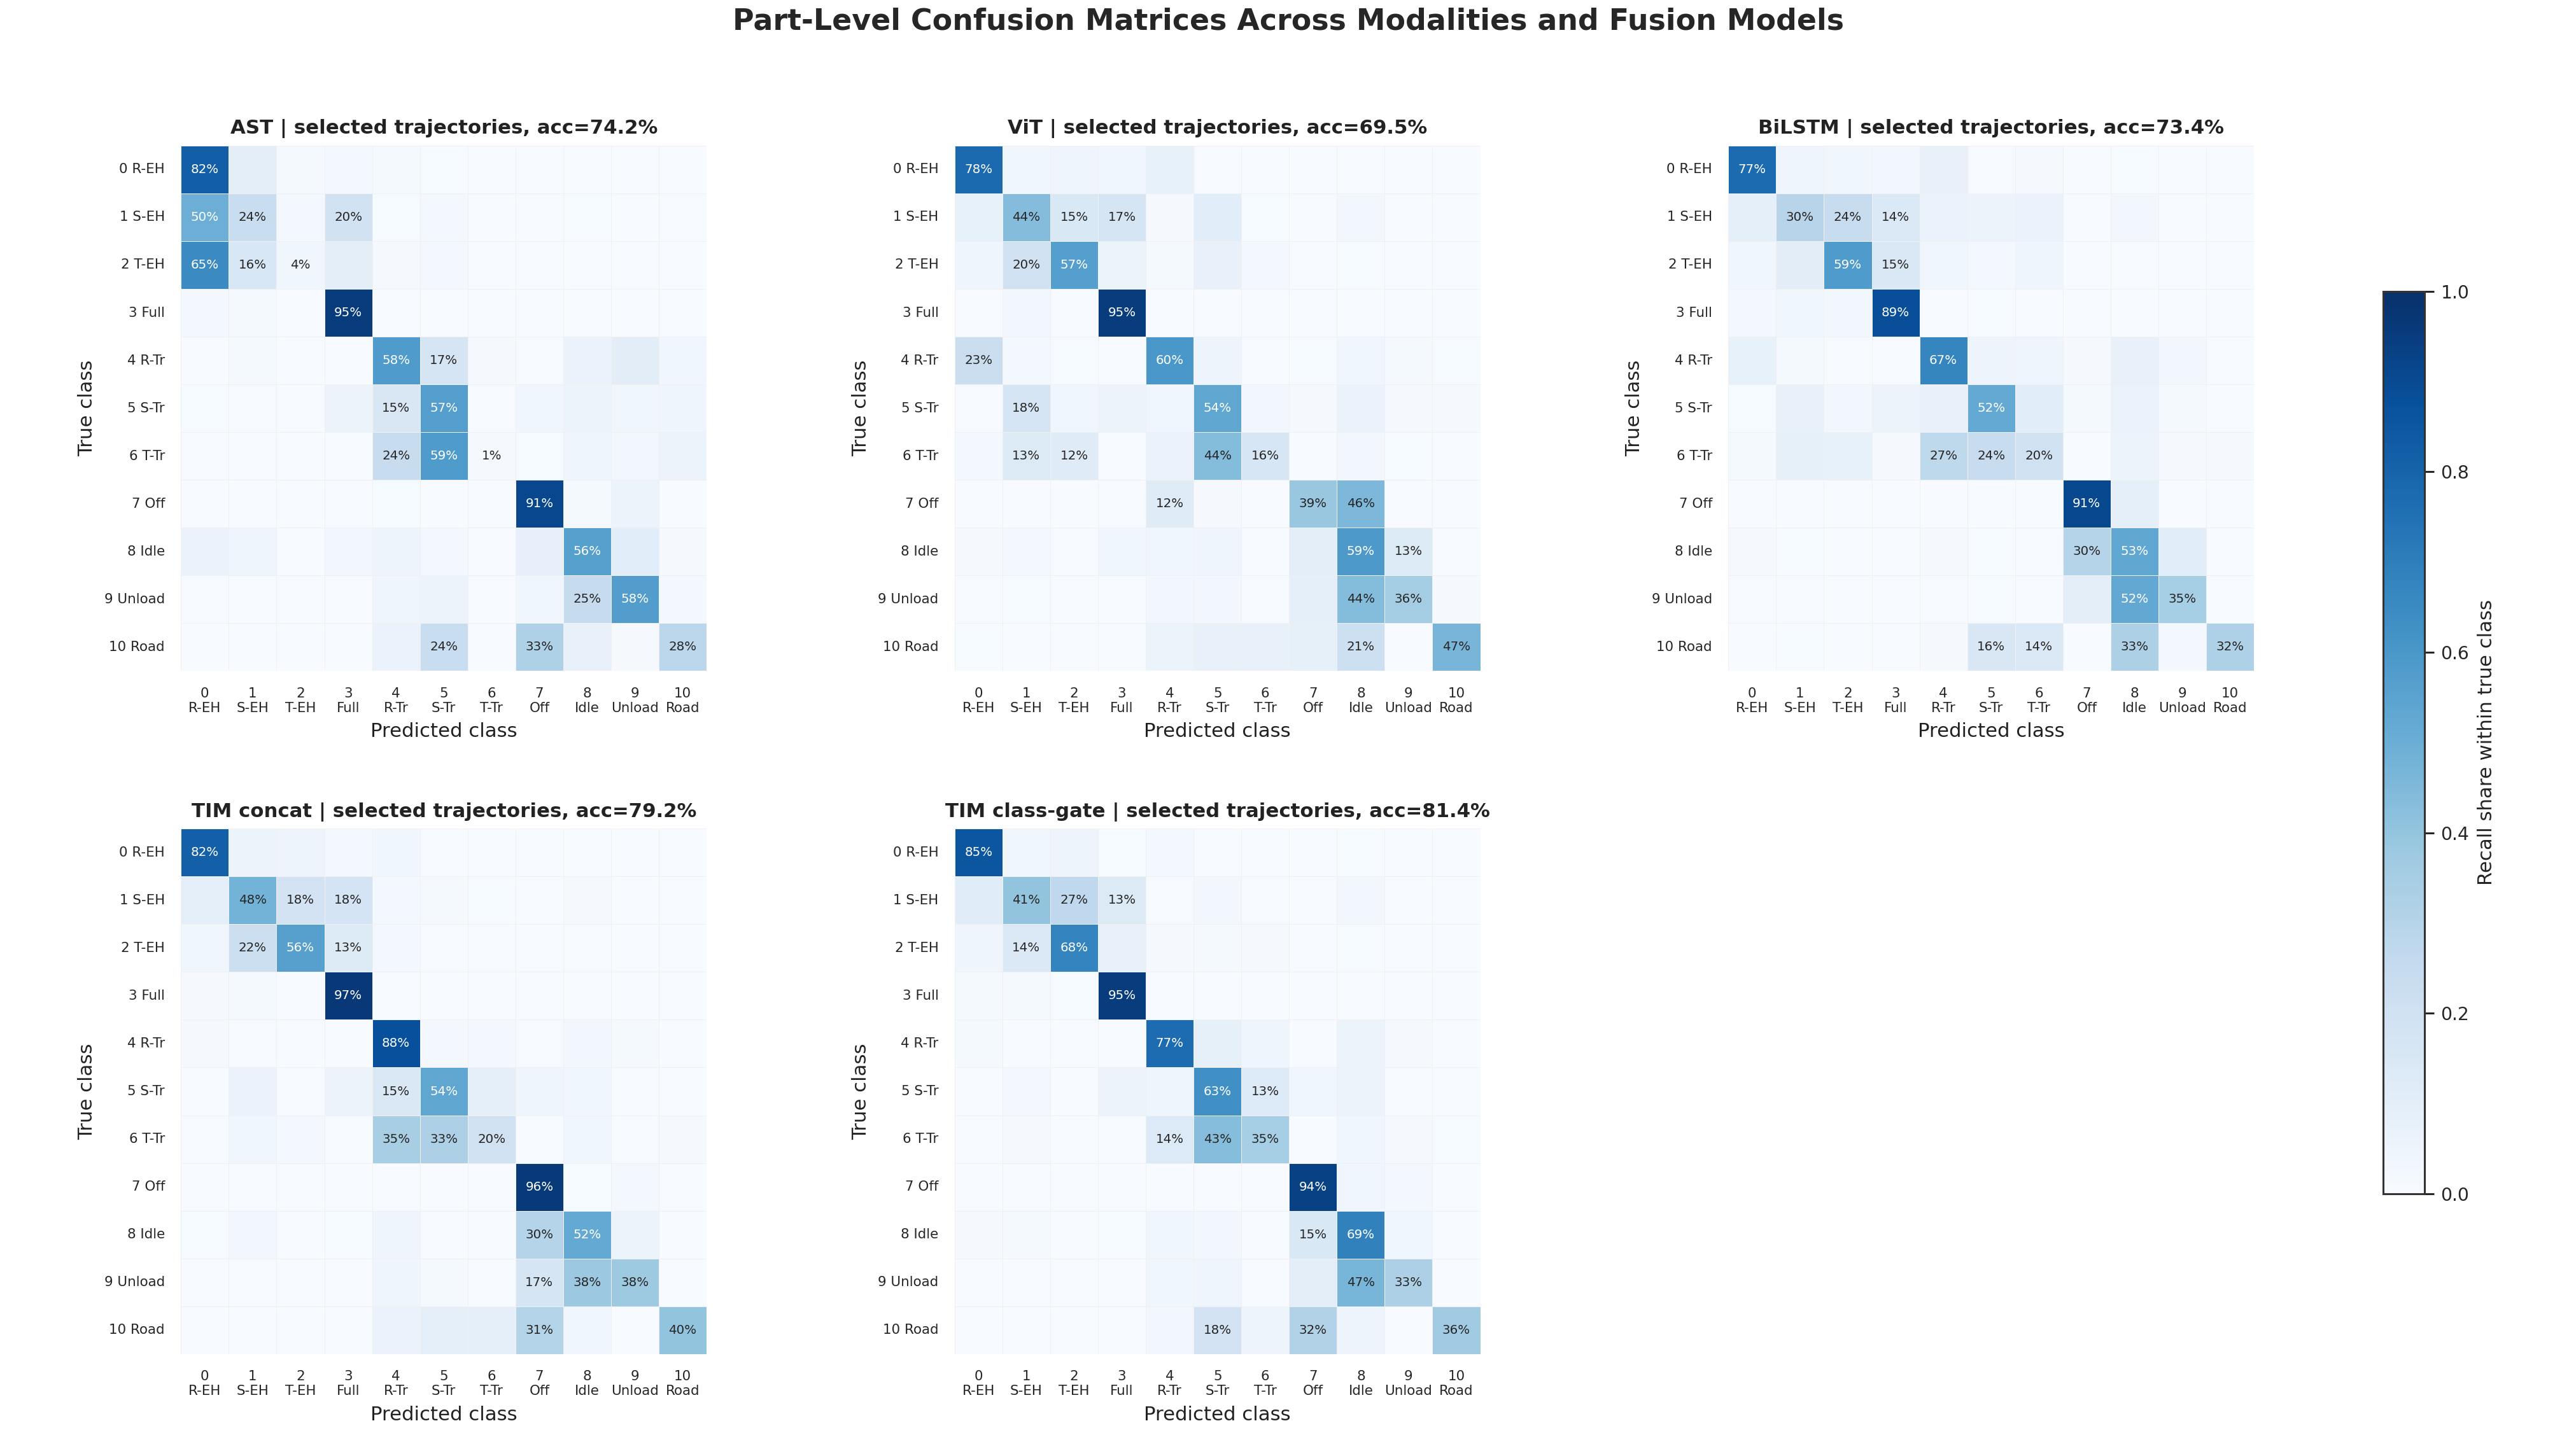
\includegraphics[width=0.99\linewidth]{fig_part_confusion_modalities.png}
\caption{Part-level confusion matrix comparison across modalities on selected held-out trajectories. Values are row-normalized recall shares within each true class. The comparison shows how different modalities fail on different behavior groups and why the trimodal model improves the overall diagonal structure.}
\label{fig:part_confusion_modalities}
\end{figure}

\Cref{fig:part_misclassification_heatmaps} focuses on off-diagonal errors for a representative trajectory selected by the criterion above. The heatmaps make the role of fusion more explicit: single modalities often concentrate errors in different class groups, direct concatenation reduces part of these errors, and TIM class-gate further reduces the largest remaining error cells.

\begin{figure}[p]
\centering
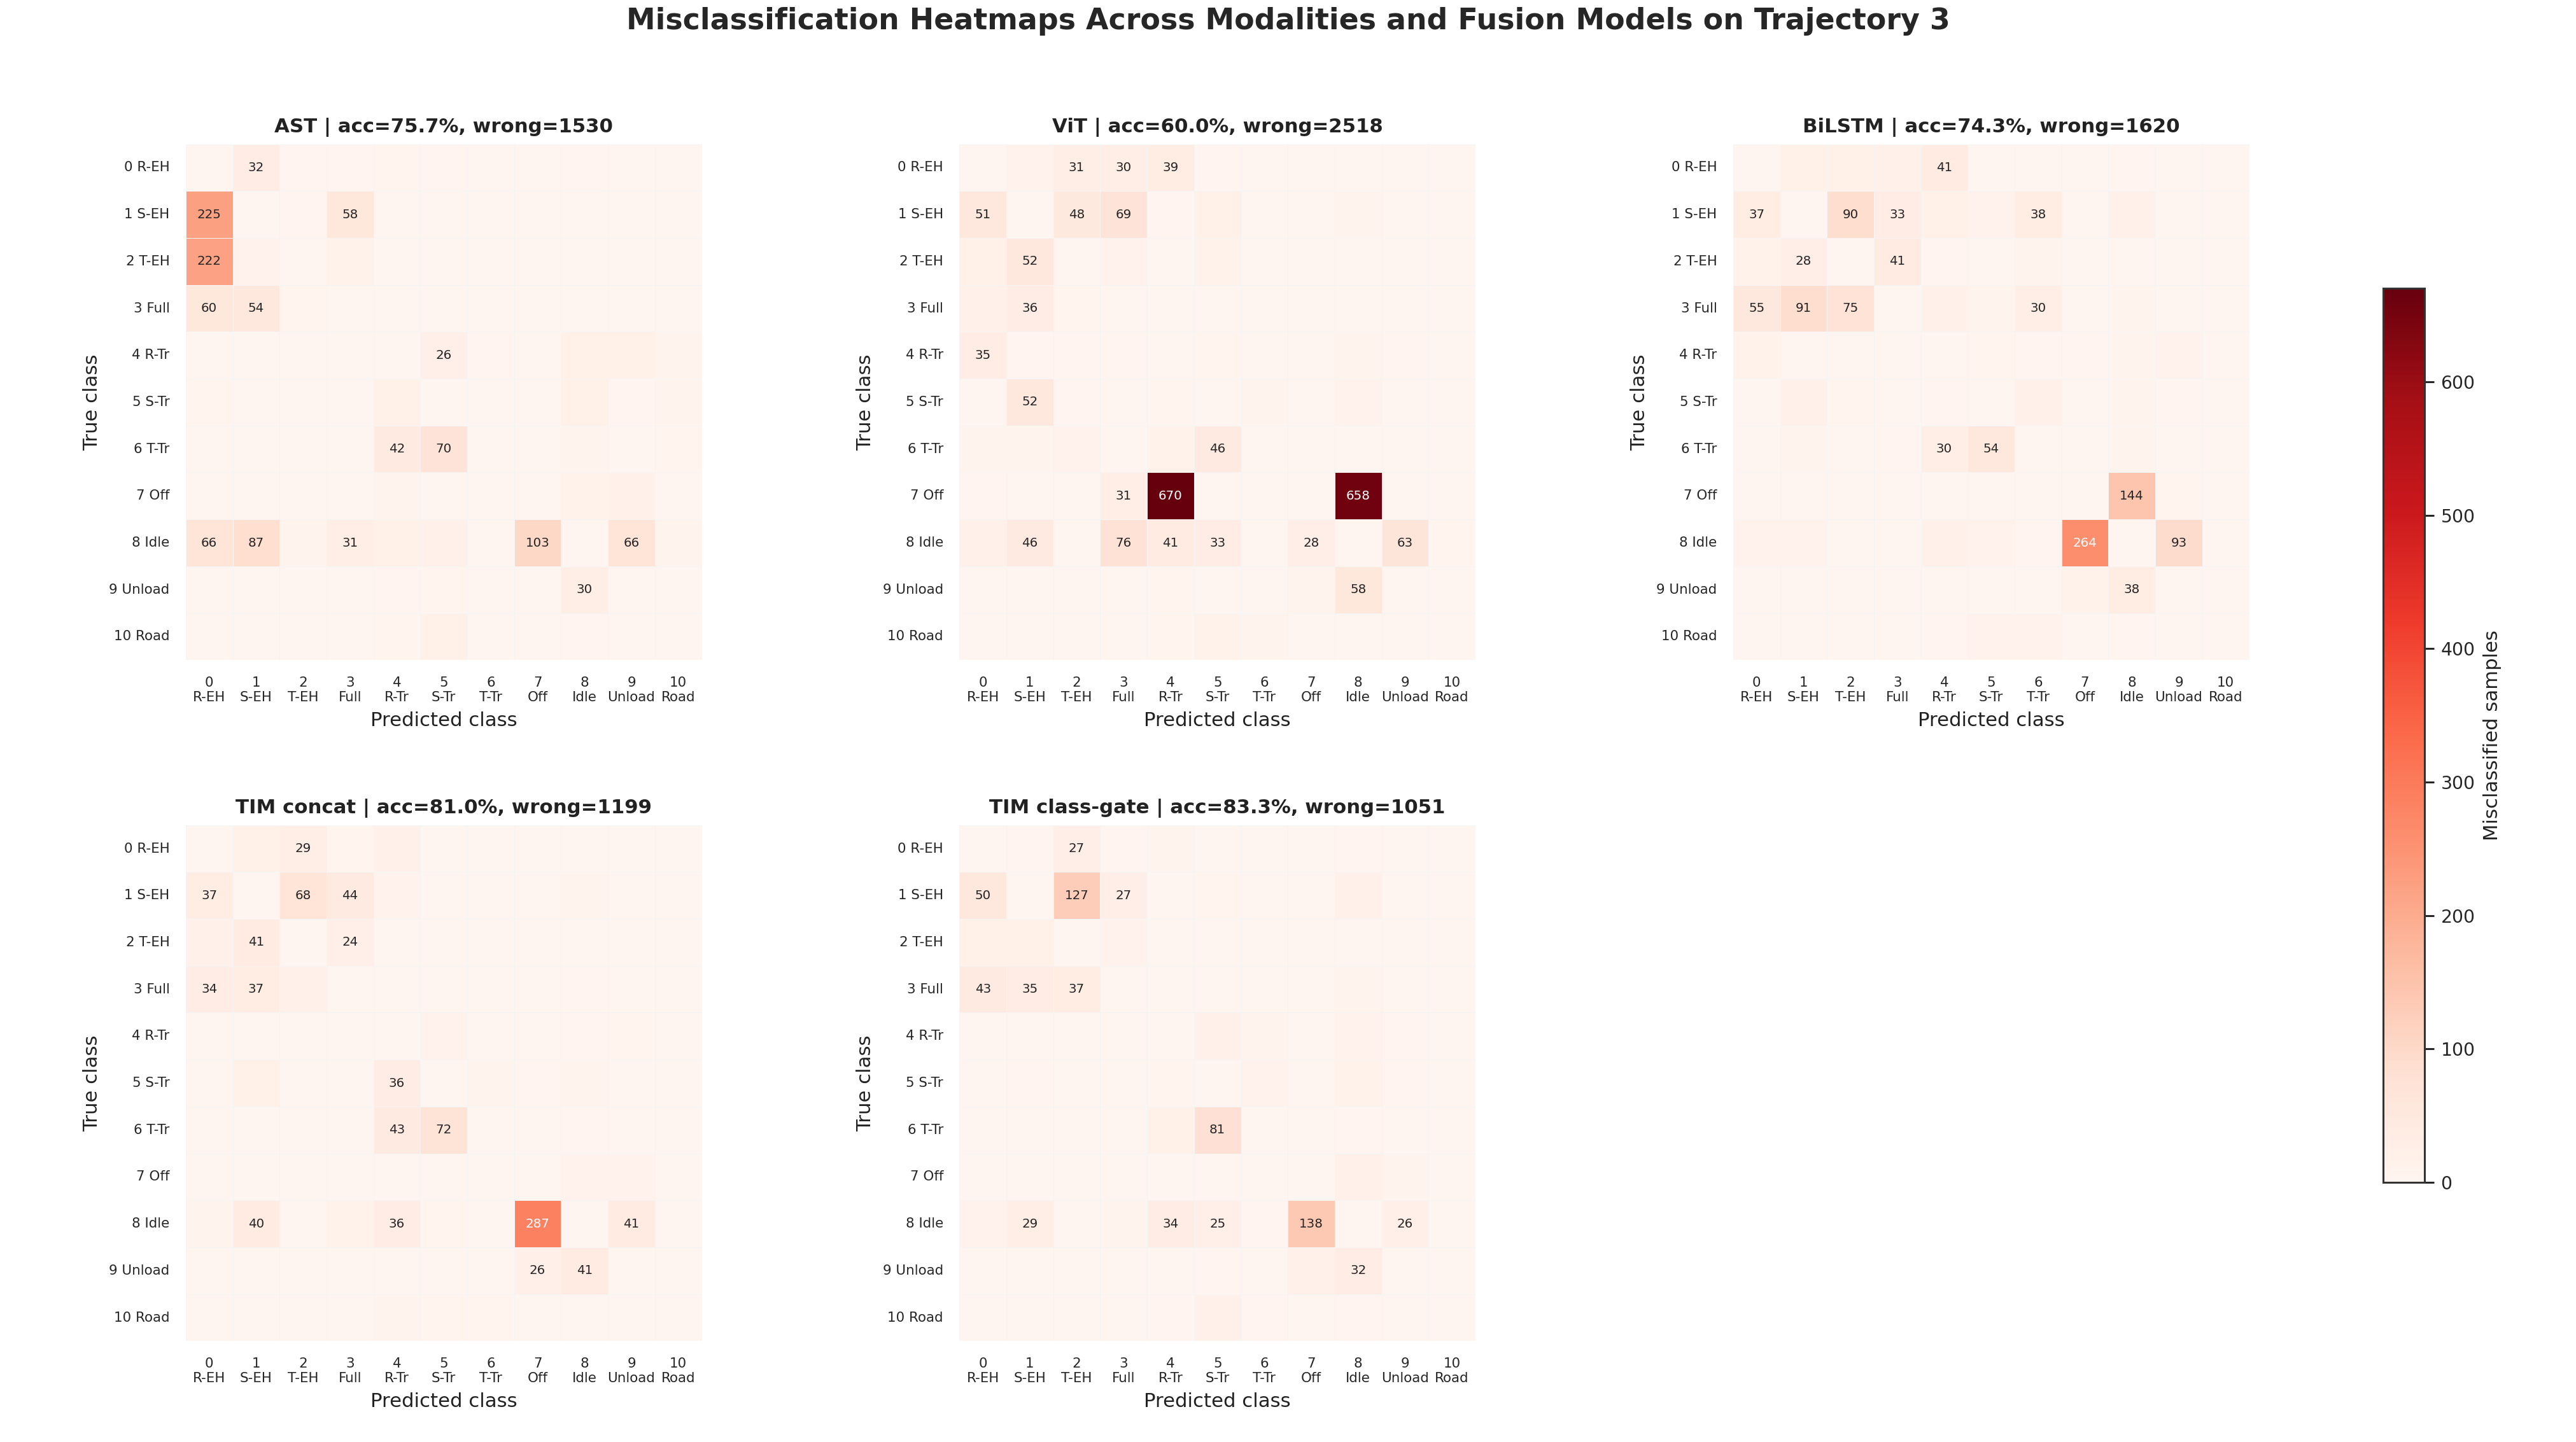
\includegraphics[width=0.99\linewidth]{fig_part_misclassification_heatmaps.png}
\caption{Misclassification heatmap comparison across modalities and fusion models on a representative held-out trajectory. Diagonal cells are removed so that the figure only reports wrong true--predicted class pairs. The representative trajectory is selected to highlight where multimodal fusion most clearly improves over the strongest single-modality baseline.}
\label{fig:part_misclassification_heatmaps}
\end{figure}

\Cref{fig:part_error_hotspots} visualizes a zoomed spatial segment rather than the full trajectory. The selected window covers a contiguous region where all models make some correct predictions, but the error density differs substantially. Plotting the same longitude--latitude window for all modalities and fusion models makes the spatial effect explicit: TIM class-gate retains a much cleaner trajectory with fewer wrong locations, whereas the unimodal branches and direct concatenation produce denser error clusters.

\begin{figure}[p]
\centering
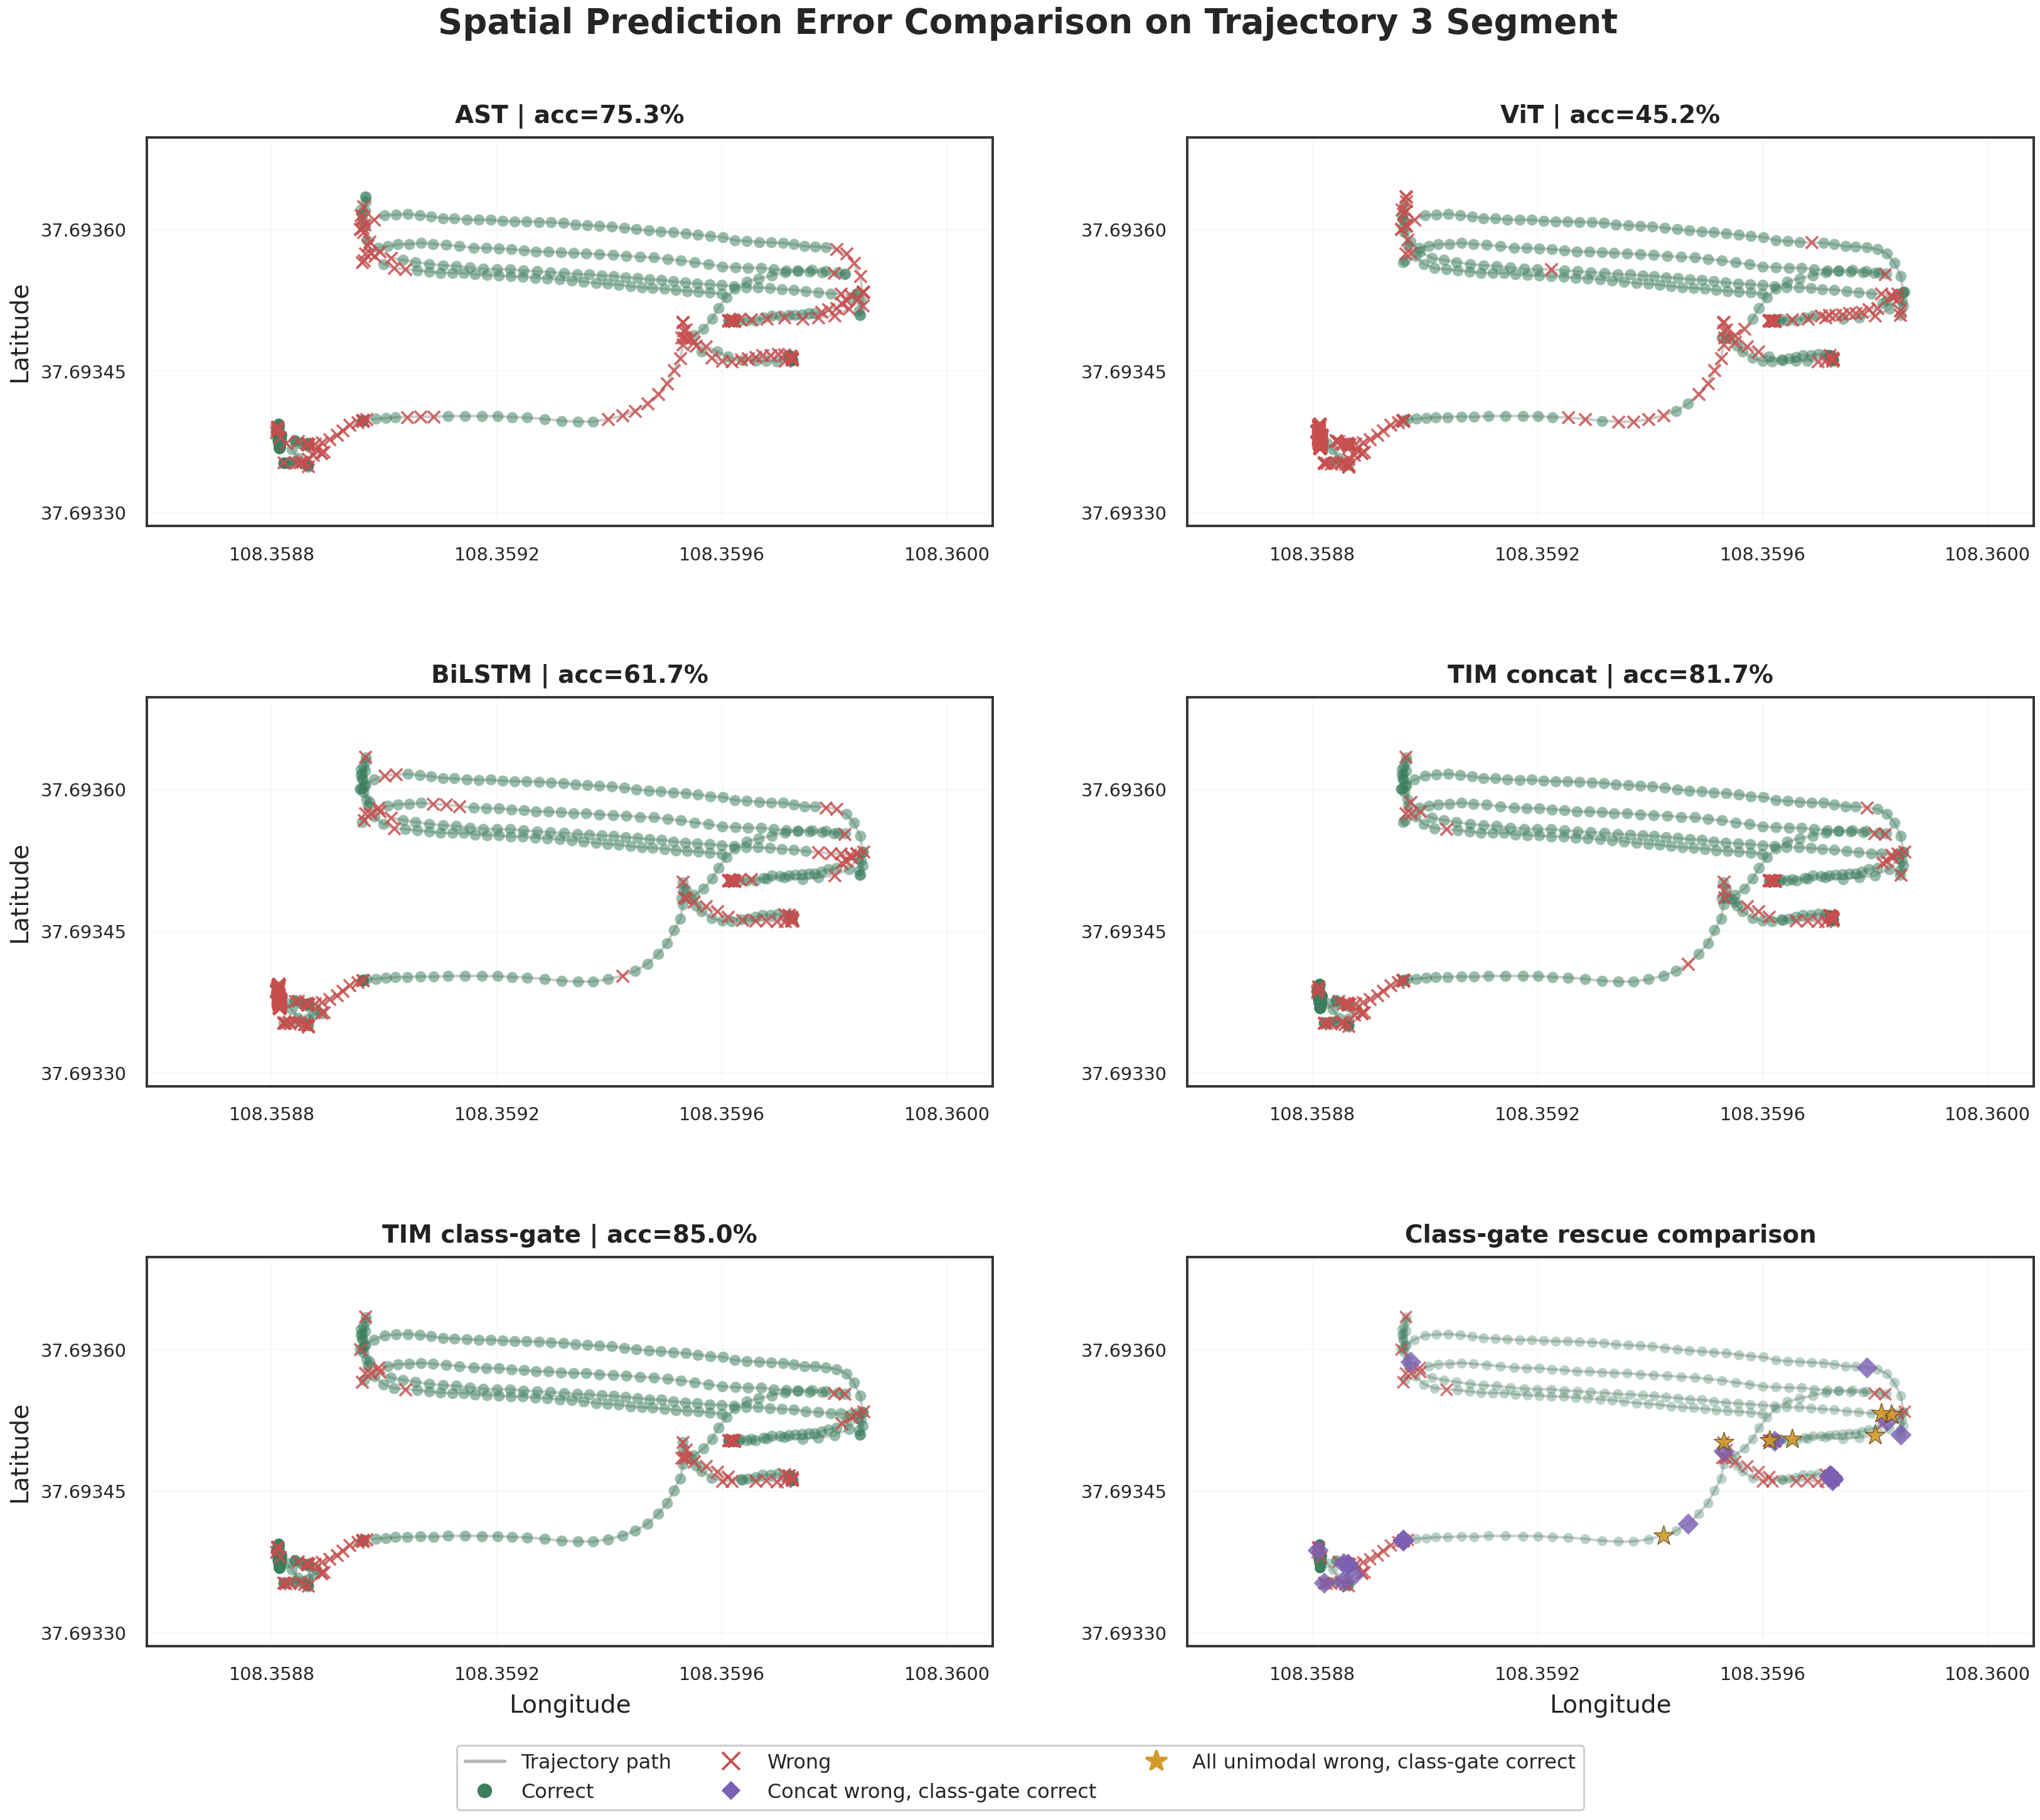
\includegraphics[width=0.98\linewidth]{fig_part_error_hotspots.png}
\caption{Spatial prediction error comparison on a representative held-out trajectory segment. The first five panels report the same longitude--latitude window for each model, while the final panel summarizes where TIM class-gate corrects samples missed by direct concatenation or by all unimodal branches. Green points are correct predictions, red crosses are wrong predictions, and the gray line is the raw trajectory path. In this selected segment, TIM class-gate produces the cleanest error pattern among the compared models.}
\label{fig:part_error_hotspots}
\end{figure}

\Cref{fig:part_spatial_errors} reports the spatial behavior of TIM class-gate with a two-level interpretation. The title of each panel reports both operation-group accuracy and eleven-class accuracy. Colored points are correct eleven-class predictions and are colored by operation group; amber markers indicate samples assigned to the correct group but the wrong subclass; red crosses indicate errors at the operation-group level. This separates semantic group recognition from fine-grained subclass residuals and avoids treating all subclass confusions as equally severe spatial failures.

\begin{figure}[p]
\centering
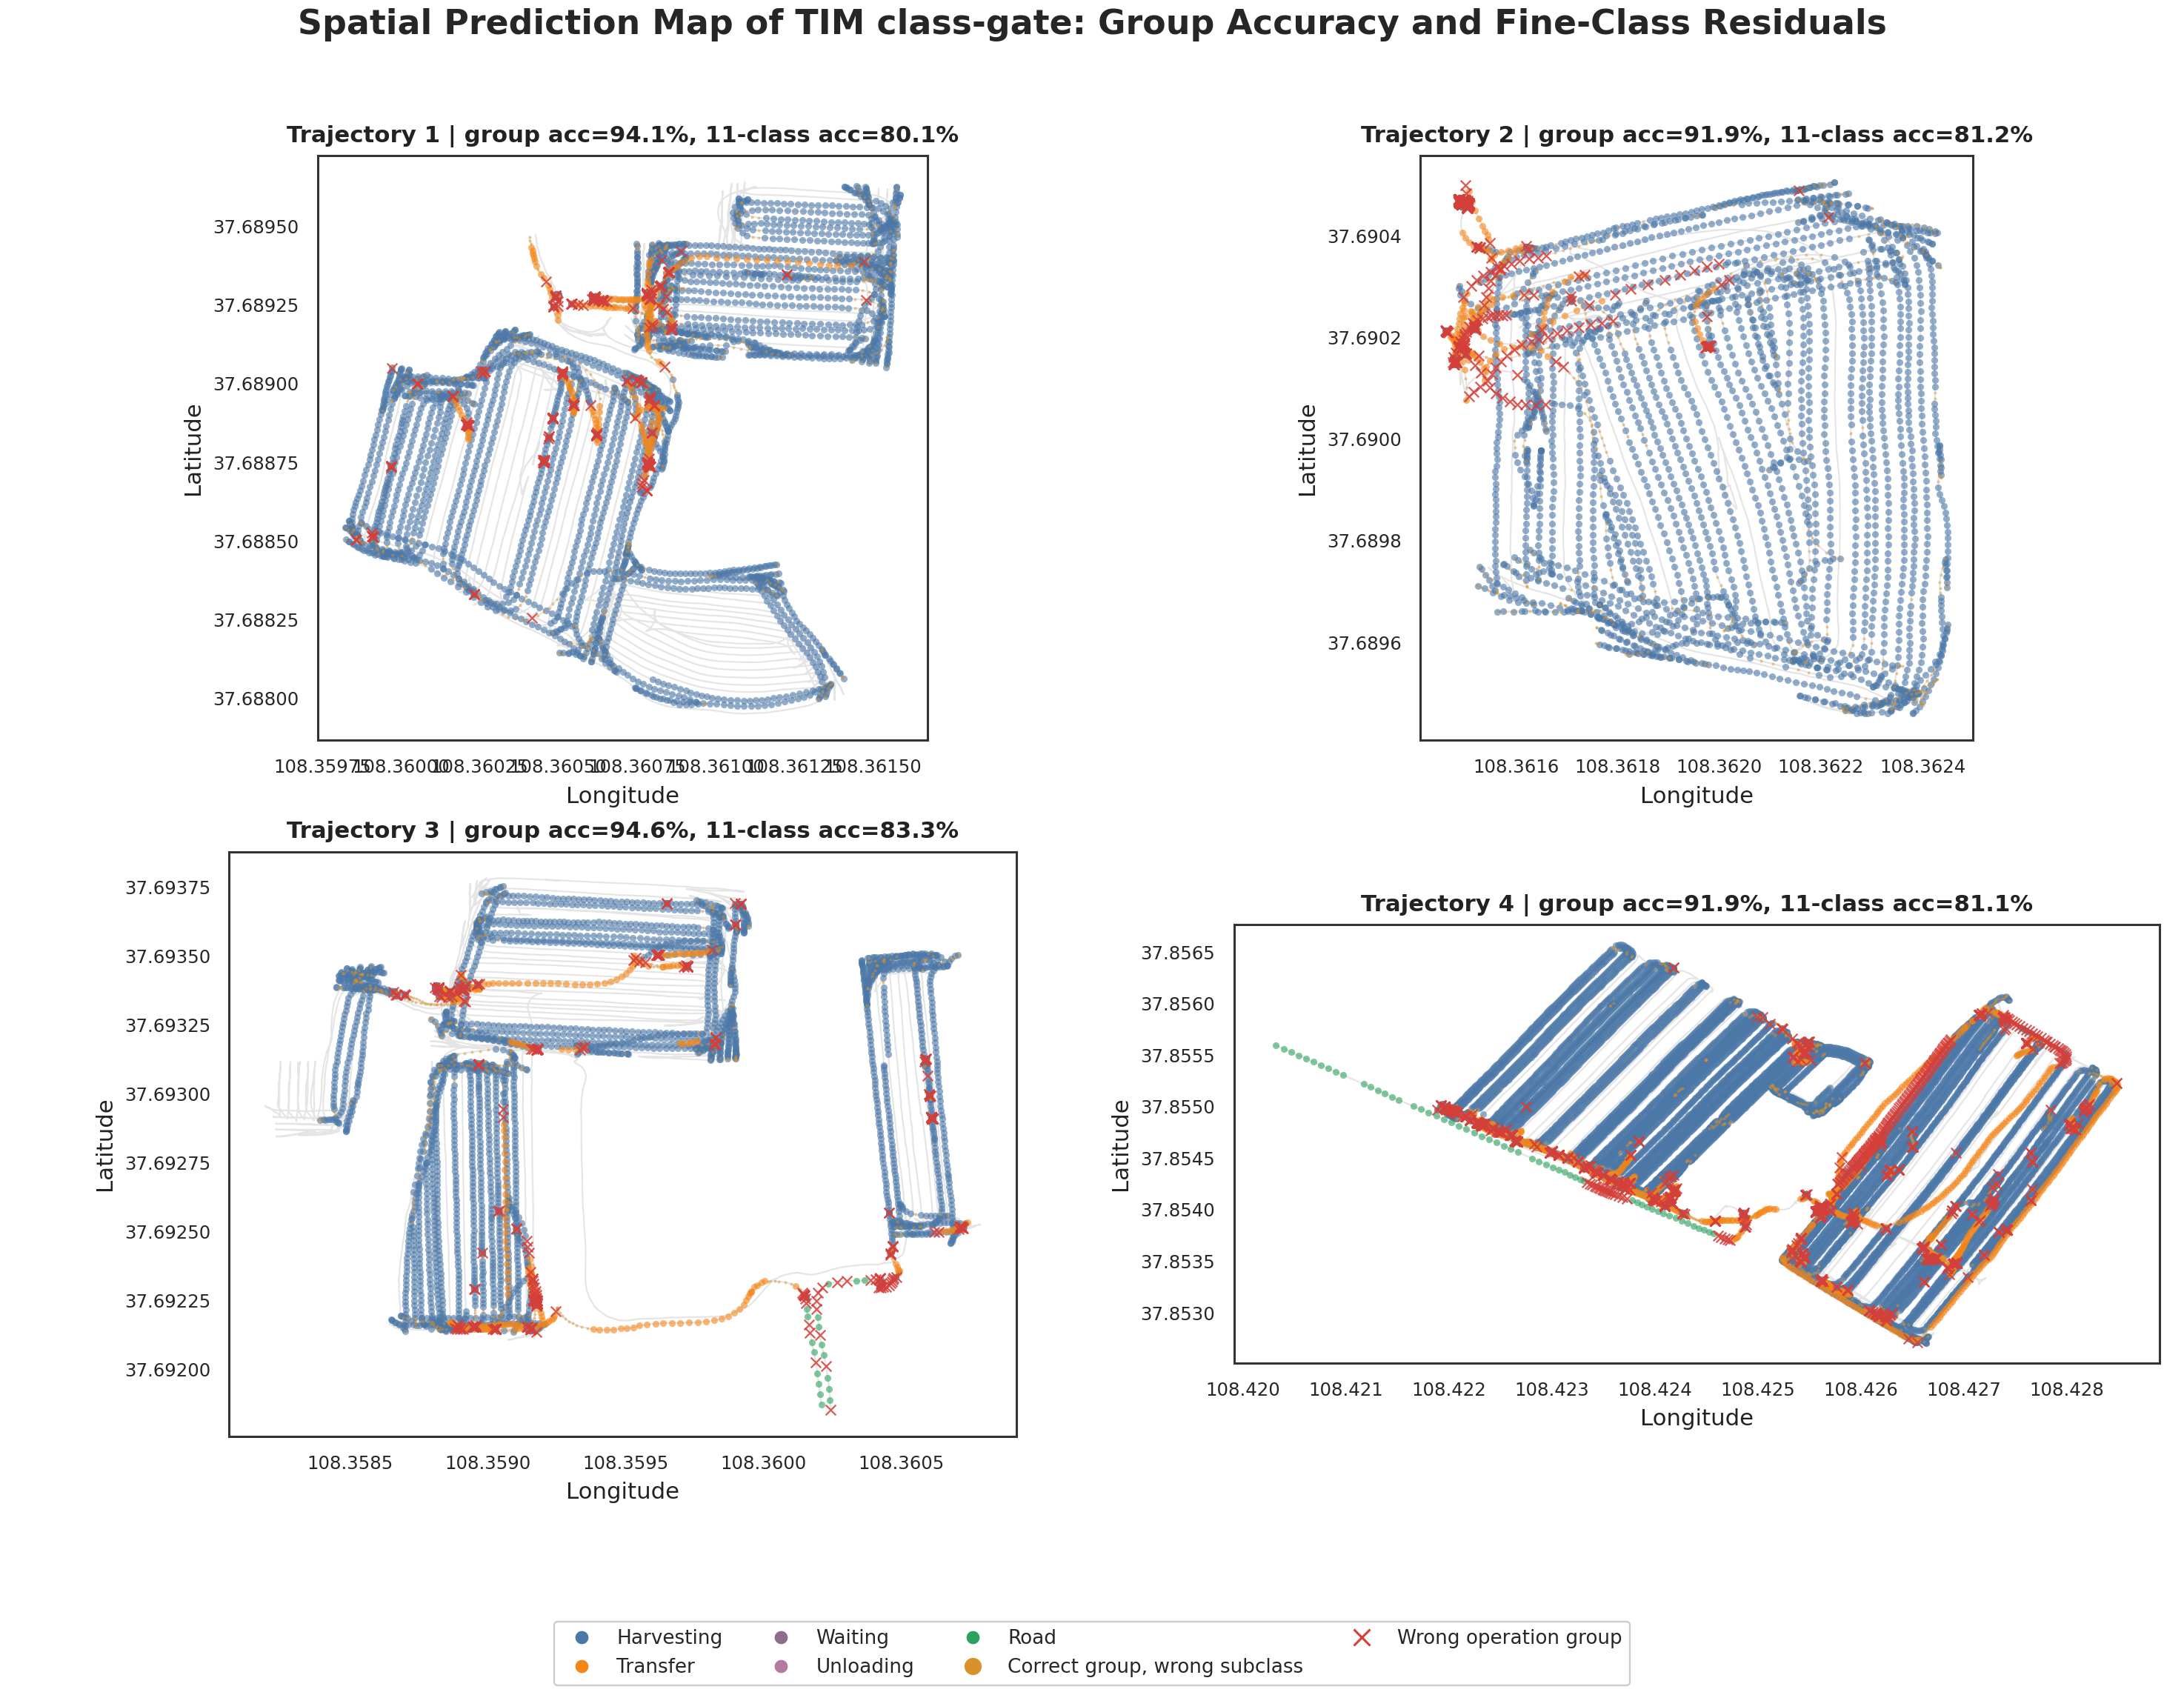
\includegraphics[width=0.98\linewidth]{fig_part_spatial_errors.png}
\caption{Spatial prediction map of TIM class-gate with operation-group accuracy and fine-class residuals. Colored points denote correct eleven-class predictions and are colored by operation group; amber markers denote correct-group but wrong-subclass predictions; red crosses denote wrong operation-group predictions. Road driving is shown in green.}
\label{fig:part_spatial_errors}
\end{figure}

\Cref{fig:part_timeline_modalities} compares temporal predictions across modalities and fusion models on a dense interval from a representative trajectory. This view shows the practical effect of multimodal fusion at the sequence level: the class-gate prediction strip is closer to the true strip and has fewer red wrong-prediction intervals than the single-modality baselines and direct concatenation.

\begin{figure}[p]
\centering
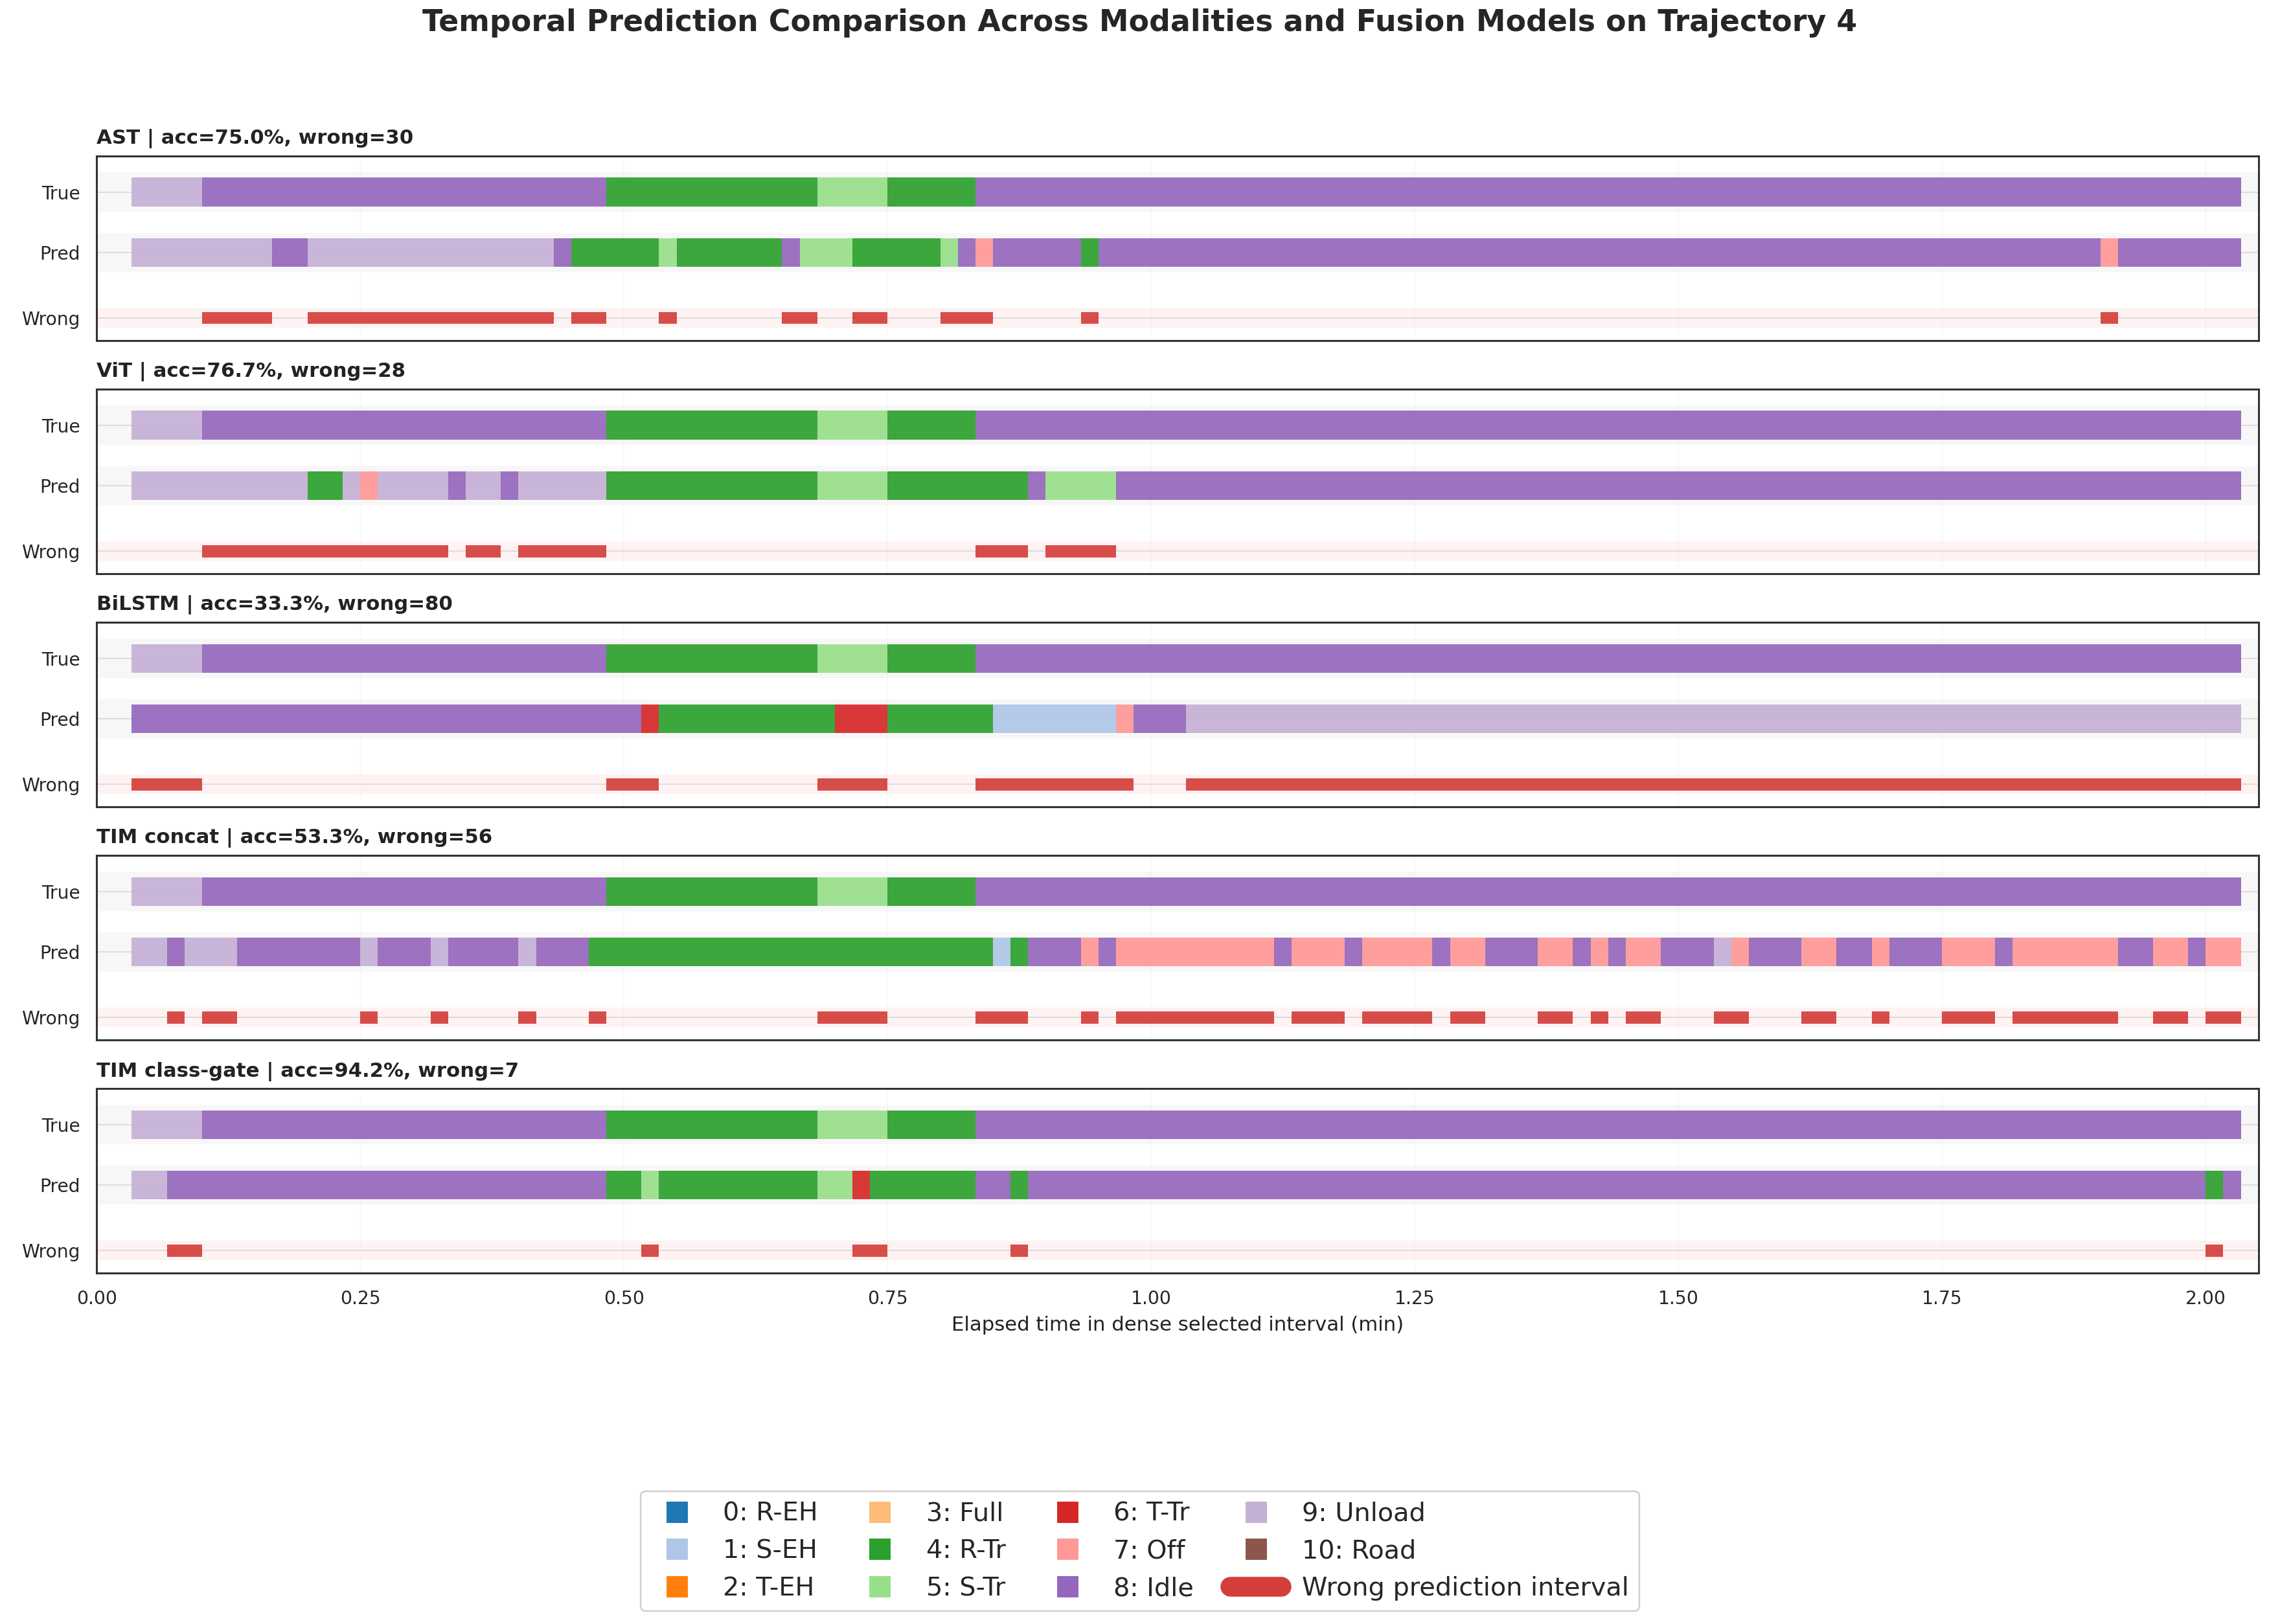
\includegraphics[width=0.98\linewidth]{fig_part_timeline_modalities.png}
\caption{Temporal prediction comparison across modalities and fusion models on a dense selected held-out trajectory interval. Each panel shows the true class sequence, the predicted class sequence, and the wrong-prediction band for the same observed time span. The horizontal axis is cropped to the portion containing prediction samples so that temporal errors can be compared without empty padding. TIM class-gate reaches 94.2\% local accuracy in this interval, compared with 75.0\% for AST, 76.7\% for ViT, 33.3\% for BiLSTM, and 53.3\% for direct TIM concat.}
\label{fig:part_timeline_modalities}
\end{figure}

\Cref{fig:part_timeline} provides the corresponding temporal view for TIM class-gate on all selected diagnostic parts. The true and predicted class strips show that many errors occur in short transition intervals rather than throughout entire operation segments. This supports the need for transition-aware temporal modeling, especially for turning empty harvesting, turning transfer, idling waiting, and unloading.

\begin{figure}[p]
\centering
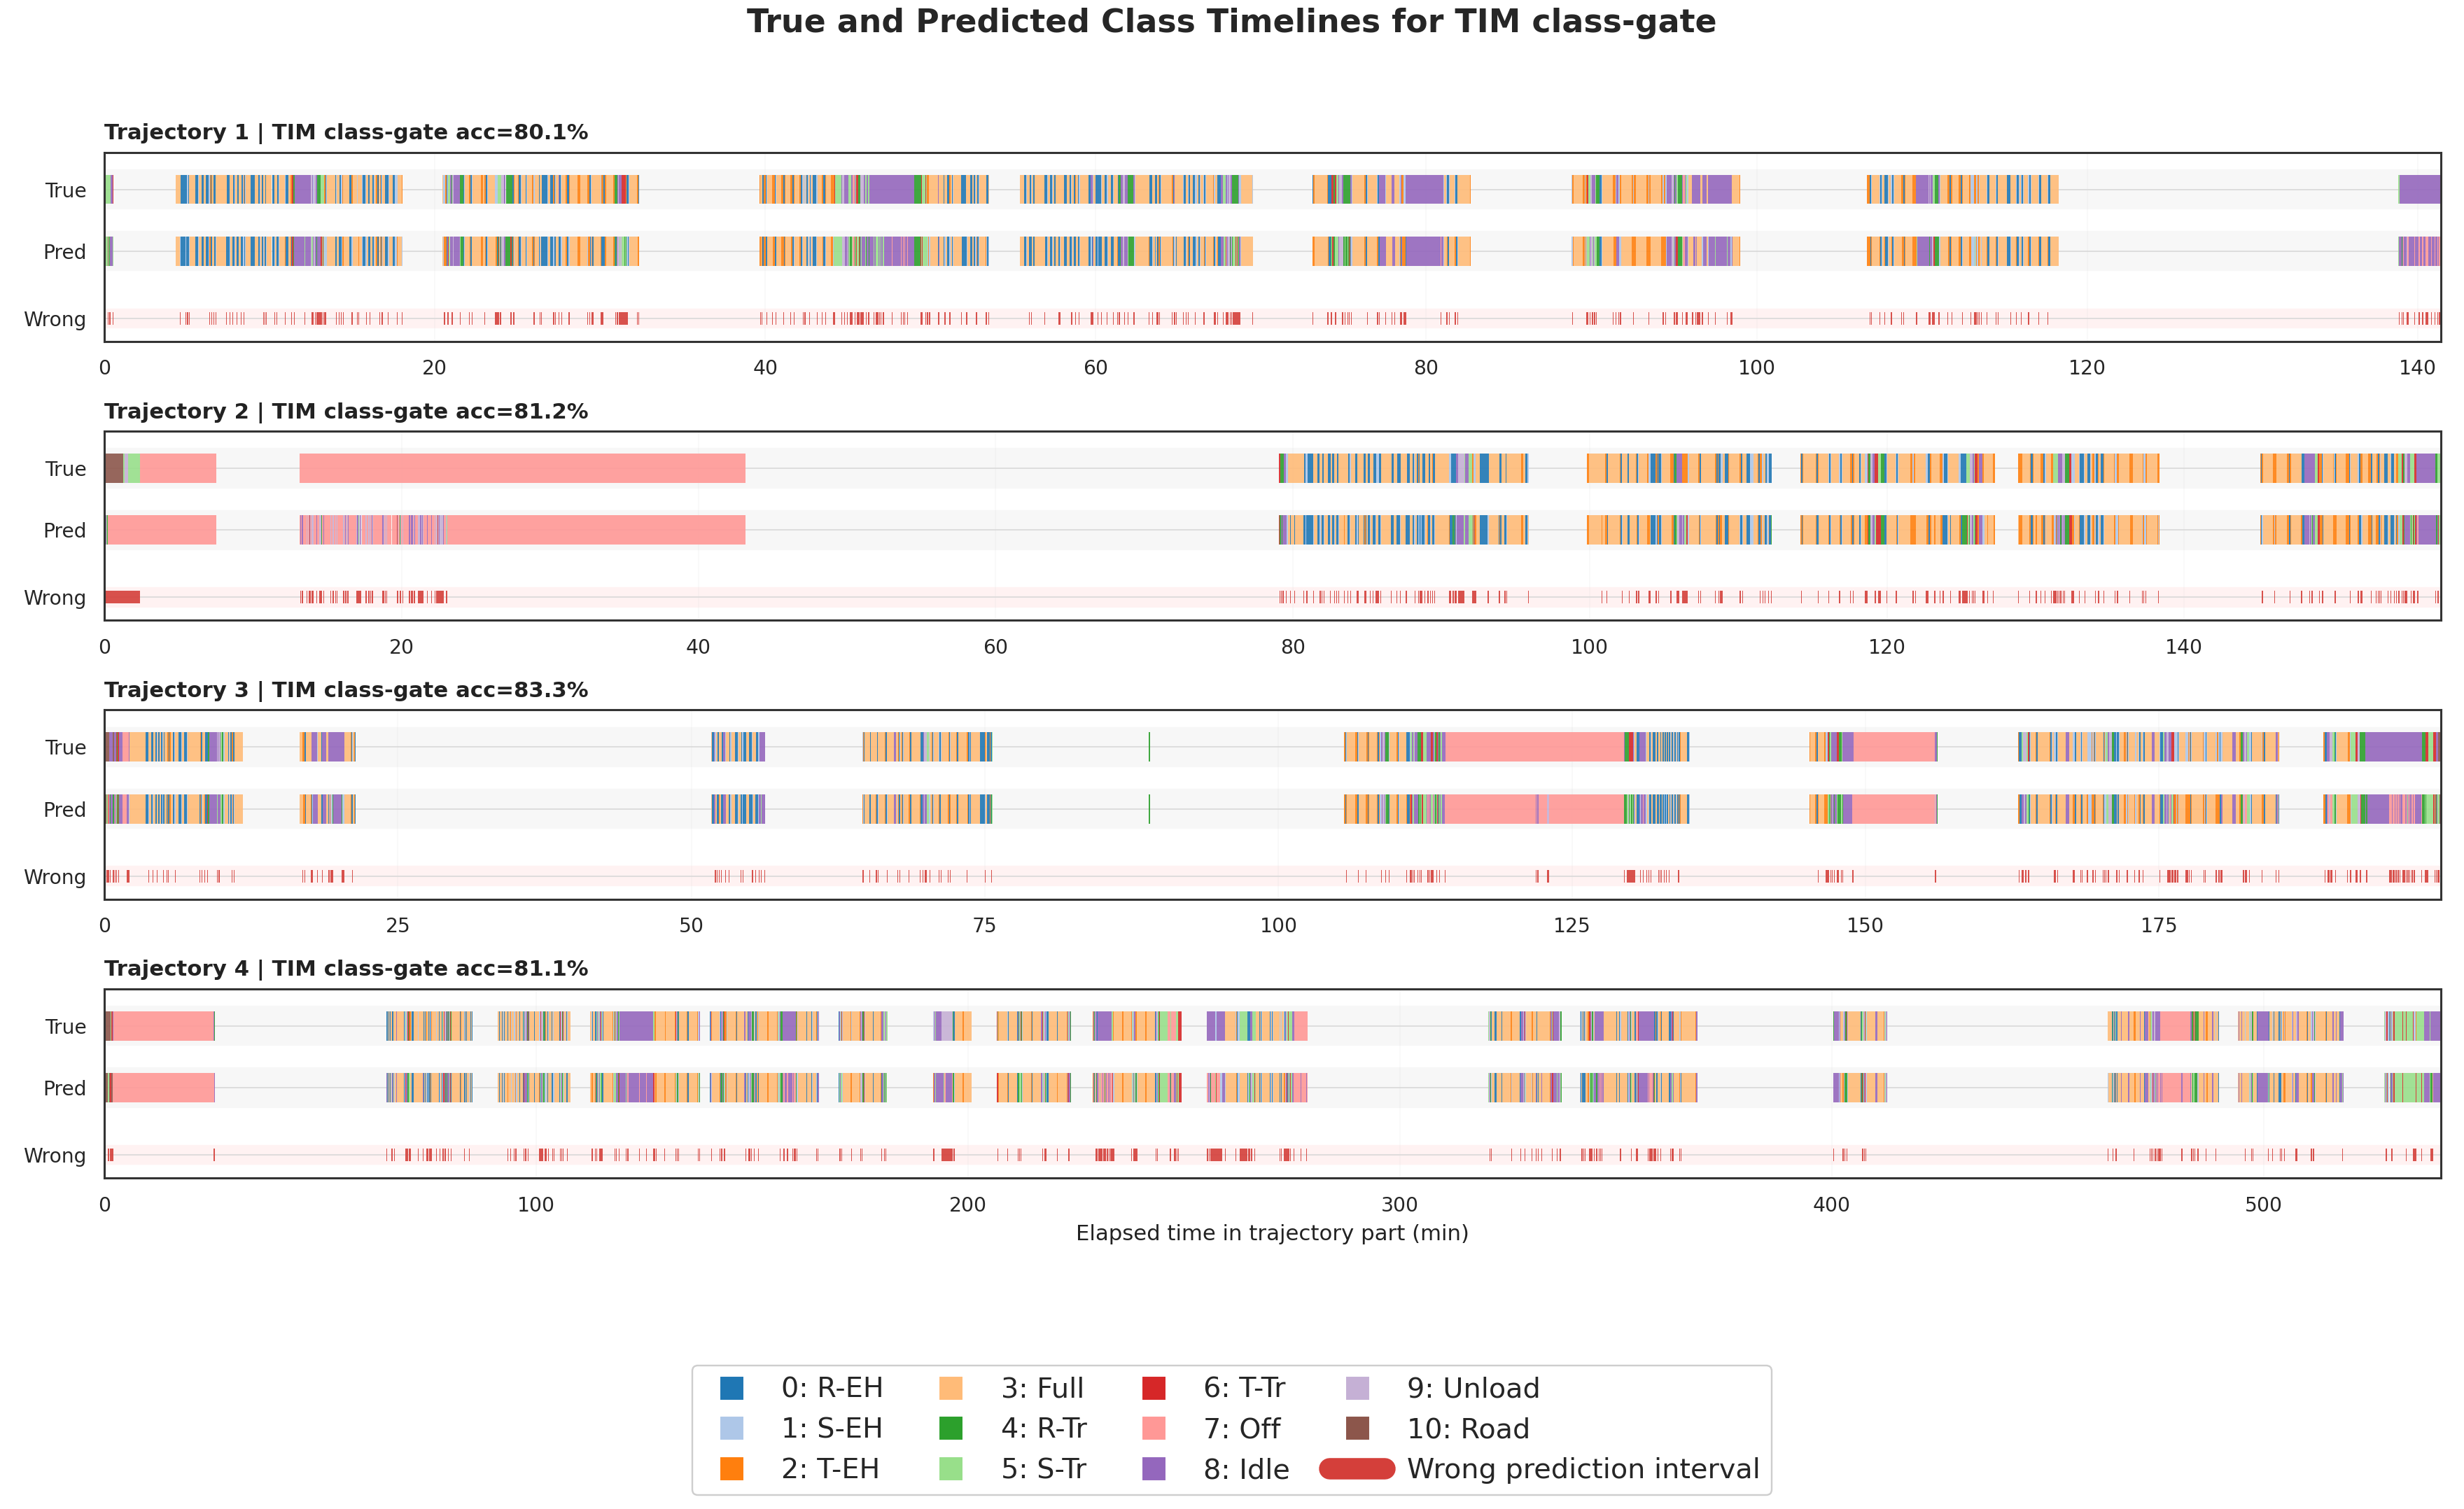
\includegraphics[width=0.98\linewidth]{fig_part_true_pred_timeline.png}
\caption{True and predicted class timelines for TIM class-gate on the selected trajectory parts. Red bands mark wrong-prediction intervals. The timeline view shows that remaining errors often occur near short transitions and ambiguous process-state changes rather than being uniformly distributed across each trajectory.}
\label{fig:part_timeline}
\end{figure}
\FloatBarrier

\section{Discussion}
\label{sec:discussion}

The experimental results show that synchronized BiLSTM trajectory, ViT visual, and AST audio signals provide complementary information for \task{}. This supports the central assumption of the study: fine-grained combine-harvester states cannot be reliably described by spatial-temporal motion alone because visually and mechanically different operations may share similar rows, speeds, stops, passes, and turns. Direct trimodal concatenation improves the fixed-seed macro-F1 by 6.56 percentage points over BiLSTM and by 14.62 points over AST, indicating that the gain is not only an accuracy effect from frequent classes but also a more balanced improvement across the eleven-class taxonomy. The proposed class-adaptive gate further improves macro-F1 by 2.44 points over concatenation, reaching 63.64\% macro-F1 and 81.36\% accuracy.

The per-class results further explain why each modality is useful. BiLSTM provides spatial continuity, direction, turning behavior, and transfer movement, which are essential for reverse transfer and straight transfer. ViT provides crop contact, road surface, visible harvesting conditions, and field-road context, which benefits empty harvesting and road driving. AST provides engine response, load variation, and working-component engagement, which explains its strong performance on full-load harvesting, engine-off waiting, idling waiting, and unloading. These findings are consistent with the practical harvesting workflow and show that multimodal sensing is not only a model-level improvement but also an operationally interpretable extension of trajectory-only classification.

At the same time, the fusion ablation reveals both the value and the limitation of class-adaptive gating. Compared with concatenation, the gate improves turning transfer by 11.74 F1 points and idling waiting by 9.60 points, and it reduces the dominant idling waiting $\rightarrow$ engine-off waiting error by 791 samples. This supports the design choice of keeping modality-specific logits before the final decision. However, unloading and road driving remain below their best single-modality baselines. These classes are either strongly process-dominated or rare in the current split, so the learned gate can still dilute the most reliable modality. This motivates future constraints on class-wise gate weights or prior-guided fusion for rare and audio-dominant states.

The dataset also reflects naturally imbalanced agricultural production rather than an artificially balanced benchmark. Full-load harvesting and waiting occupy large temporal proportions, whereas turning transfer and road driving are minority classes. This imbalance explains why accuracy alone can be misleading: AST reaches 74.24\% accuracy but only 46.57\% macro-F1 because it performs well on major process classes while failing on several minority motion classes. Macro-F1, per-class recall, and trajectory-level diagnostics are therefore necessary for evaluating the practical usefulness of \task{} models.

Several limitations remain. First, the final trimodal comparison currently uses a fixed seed, while only the BiLSTM sequence-length ablation has been evaluated across multiple seeds. Additional final-suite seeds are needed before making strong statistical claims. Second, the study is restricted to combine harvesters during maize harvest operations in three regions; cross-machine, cross-crop, and cross-season generalization remains to be tested. Third, the current multimodal model uses synchronized observations but does not explicitly model transition boundaries or class-neighborhood structure, which contributes to errors such as turning transfer being confused with reverse or straight transfer. Future work should therefore combine the class-adaptive gate with transition-aware temporal modeling and imbalance-aware objectives for minority operation classes.

\section{Conclusion}
\label{sec:conclusion}

This paper presents TIM, a trajectory-image-audio multimodal model for eleven-class \task{}. The study is built on a synchronized real-world combine-harvester dataset and a matched causal temporal protocol: 128-second trajectory context, nine nearest causal ViT frames, AST-based audio spectrogram encoding, and class-adaptive logit-level trimodal fusion.

The completed BiLSTM sequence-length ablation shows that 128 seconds is the best trajectory context among 64, 128, 256, and 512 seconds, reaching a mean macro-F1 of 54.64\% across four seeds. Direct trimodal concatenation demonstrates the value of synchronized multimodal sensing, improving macro-F1 by 6.56 percentage points over the strongest unimodal baseline. The proposed class-adaptive gate further improves the fixed-seed trimodal result to 81.36\% accuracy, 63.64\% macro-F1, and 81.01\% weighted-F1.

The fusion ablation shows why the current model replaces conventional concatenation with class-adaptive fusion. The gate improves turning transfer, reverse transfer, idling waiting, and turning empty harvesting, and it substantially reduces the largest waiting-state confusion. The remaining errors are concentrated in unloading, road driving, and fine-grained transfer substates. Future work should therefore combine class-adaptive fusion with transition-aware temporal modeling, imbalance-aware objectives, and gate constraints for rare or strongly audio-dominant classes.


\bibliographystyle{elsarticle-harv}
\bibliography{references}

\end{document}
